\documentclass[useAMS,usenatbib,a4paper]{mn2e}
\usepackage{graphicx}
\usepackage{aas_macros}
\usepackage{multirow}
\usepackage[draft]{hyperref} % draft option seems to fix some hyperref issues
%\usepackage{hyperref}
     
\title[Mid-infrared spectroscopy of M31]{Mid-infrared spectroscopy of the Andromeda galaxy}
\author[D. Hemachandra et al.]
{D. Hemachandra$^{1}$\thanks{E-mail: dhemacha@uwo.ca},
P. Barmby$^{1}$, 
E. Peeters$^{1}$, 
S.P. Willner$^{2}$, 
M.L.N. Ashby$^{2}$,
H.A. Smith$^{2}$, 
\newauthor 
K.D. Gordon$^{3}$,
D.A. Smith$^{3}$,
and
G.G. Fazio$^{2}$\\
$^{1}$Department of Physics and Astronomy, University of Western Ontario, London, ON, N6A 3K7, Canada\\
$^{2}$Harvard-Smithsonian Center for Astrophysics, Cambridge, MA 02138, USA\\
$^{3}$Space Telescope Science Institute, 3700 San Martin Drive, Baltimore, MD 21218, USA
}


\begin{document}

\date{}

\maketitle

\label{firstpage}

\begin{abstract}
We present {\sl Spitzer}/Infrared Spectrograph 5--21~$\mu$m spectroscopic maps towards 12 regions in the Andromeda galaxy (M31). 
These regions include the nucleus, bulge, an active region in the star-forming ring, and 9 other regions chosen to cover a range of mid-to-far-infrared colours. 
PAH feature ratios (6.2~$\mu$m and 7.7~$\mu$m features compared to the 11.3~$\mu$m feature) 
measured from our extracted M31 spectra are consistent with those seen in other nearby galaxies. 
Our  observations did not reproduce the suppressed 6--8~$\mu$m features and enhanced 11.3~$\mu$m feature seen  
with the ISOCAM instrument on the Infrared Space Observatory. 
The equivalent widths of the main PAH 
features decrease with increasing radiation hardness, consistent with that observed for other nearby spiral and starburst galaxies. 
The nucleus does not show any PAH emission except for the 11.3~$\mu$m feature but does show strong silicate emission at 9.7~$\mu$m. 
Both of these characteristics provide evidence for a low luminosity active galactic nucleus in M31.
\end{abstract}

\begin{keywords}
galaxies: individual: M31 --
galaxies: ISM --
galaxies: nuclei --
infrared: ISM --
ISM:  molecules -- 
ISM: lines and bands
\end{keywords}



\section{Introduction}

% MLNA comments, move to correct locations
%Title: rather generic.  Can you instead say something specific about what characteristics you're describing?  Maybe mention PAHs and silicate emission?
%
%Abstract: 
%
%We present observations of the mid-IR spectra obtained from Spitzer-IRS, covering the wavelength range from 5 to 21 microns towards 12 regions in M31 
%
%-->  We present {\sl Spitzer}/Infrared Spectrograph 5--21\,$\mu$m spectra towards 12 regions in M31
%
%acronym ISOCAM not defined at first use
%
%ISOCAM spectro-imaging observations of M31 showed unusual PAH feature ratios; however, the spectra that we obtained show PAH emission between 6 - 8 microns disagreeing with the previous results from ISOCAM observations.
%
%--> Our spectra reveal PAH emission between 6 and 8 microns that is inconsistent with earlier ISO/ISOCAM observations by [REF HERE] that showed unusual PAH feature ratios.
%
%important: Later on you refer to a re-reduction of the ISOCAM data.  If that's already out there, and it refutes Cesarsky et al, then there's really no need to refer to that paper as a result that we need to confront...somebody else already did it.  In which case, the motivational part of the paper ought not to present Cesarsky et al as something that's still current.
%
%A few trivial points: e.g., and i.e., should be followed by commas in American English (e.g., the ApJ).  Elements of a paper should always be capitalized (Section, Table, Figure).  The text should be consistent about mid-IR vs mid-infrared and other such constructions.  Throughout there is a missing space after arcsec units.  Re-examine places where the word "values" appears, because it is usually not needed:  EQW values --> EQWs, flux values --> fluxes, metallicity values --> metallicities, for example.
%Table 1 would be better if it included the galactocentric radii (perhaps), and the UV intensities, metallicities, and dust temperatures (definitely) used to choose them as targets in the first place.  Also which fields were previously observed by ISO/ISOCAM.  Suggested new title: Spitzer/IRS Target Locations in M31.
%
%Table 2 should make explicit that the fluxes given are prior to color-correction
%
%How was the line of best fit derived -- did you weight by uncertainty?
%
%Can you cite others who applied *offsets* to force IRS spectra to match up, as opposed to using only multiplicative factors -- is this standard practice?
%
%The title of Sec 3 should be more specific; data analysis sounds akin to data reduction.  Sec 3 (text) needs to be much clearer as to which spectra (IRS or ISO) are being discussed.
%
%Sec 3.1, para 1, 1st sentence needs a reference, like maybe an ISO user's guide or some kind of technical memo.
%
%I suppose others may know what a Drude profile is, but this is the first I've heard of it
%
%Sec 3.2, last para.  Why do you hard-wire these parameters to exclude them entirely, if there is *some* contribution seen from them in the spectra?
%
%Do you need to number the equation in Sec 3.3, para 1.  Also, it is unclear from the text why you write it this way instead of just putting I(nu)_feature in the numerator and then having to explain your notation in the text
%
%Does PAHFIT *separately* fit an independent Gaussian to each of the atomic lines in Sec 3.4?  They are not correlated in any way?
%
%Figures 8 and 9 are really just the same figure, spread over two pages.  Is there any benefit to showing the fit residuals in each case?  The fits looks quite good BTW
%
%Table 5 has names inconsistent with other tables in the paper
%
%Fig 12 caption -- what is meant by "dividing each EQW by their weighted average over all regions."  -- why do you normalize in this way?
%
%Sec 4.3 -- I see the North region, but where is the South East one -- can it be indicated in Fig 14 somehow,  to distinguish from the noise at the edge of the mosaic?
Mid-infrared spectra provide a unique diagnostic tool to understand the physical conditions in the interstellar medium of galaxies. 
The rich range of spectral features (Polycyclic Aromatic Hydrocarbons (PAHs), atomic fine structure lines (e.g. Ne, S) and the
amorphous silicate feature centred at 9.7~$\mu$m) provide information on dust properties, radiation field and star formation. 
With the advent of infrared space telescopes, such as the Infrared Space Observatory (ISO, \citealt{Kessler1996}) and 
the {\em Spitzer} Space Telescope \citep{spitzer2004}, we have been able to well explore the infrared emission from galaxies. 

PAHs are known as the main carrier of the ubiquitous mid-IR emission bands (e.g. \citealt{Allamandola1989}, 
\citealt{Tielens2008}). They are large hydrocarbon molecules consisting of $\sim$50--100 carbon atoms. 
The main PAH features are seen at 3.3, 6.2, 7.7, 8.6, 11.3 and 12.7~$\mu $m (e.g.\citealt{Mattila1996}, \citealt{Peeters2002}), 
and these bands are due to the vibrational de-excitation of PAH molecules  through bending and stretching modes of C-H and C-C bonds \citep{Tielens:2005lr}. 
The 6 to 8 micron features are thought to originate mostly from ionized PAHs and the 3.3, 11.3, 12.7 and 17.1~$\mu$m 
emission bands from neutral PAHs \citep{Peeters2002}. 

% SPW:  I don't understand what you mean about PAH "strengths" not varying.  Ratio to starlight varies quite a lot in different galaxies; in fact it's a decent measure of specific star formation rate.  Did you mean the relative strengths of different features?  Final two sentences of this par should come later in Sec 1, after the general review.
The relative strengths of the PAH features do not vary much within normal-luminosity galaxies \citep{Smith:2007lr} or within 
massive starburst galaxies \citep{Brandl2006}. But they do change significantly close to active galactic nuclei where the 
strength of PAHs gets weaker (\citealt{Roche1991}, \citealt{Smith:2007lr}). \citet{Smith:2007lr}  found that the mid-IR 
spectra from weak AGNs show suppressed 6 to 8~$\mu$m PAH features but are bright at 11.3~$\mu$m. 
A possible explanation for this behaviour is that AGNs alter the grain composition by selective destruction of small ionized PAHs. 
% SPW: Final two sentences of this par should come later in Sec 1, after the general review.
ISOCAM spectro-imaging observations of M31\citep{1998Cesarsky} showed that four regions including the nucleus and bulge 
of this galaxy have very odd PAH spectra, bright at 11.3 and 12.7~$\mu$m but lacking the usual 6.2, 7.7, and 8.6 micron bands. 
Investigating this unusual PAH emission was the main motivation for the work described in this paper. 

% SPW: which are "these galaxies" in which PAH EQW decreases?  Par overall is a bit confusing, especially given the previous par has asserted that something about PAH doesn't vary. 
Previous studies of nearby galaxies indicate that metallicity and radiation hardness correlate with PAH equivalent widths (EQWs). 
\citet{Smith:2007lr} and \citet{Engelbracht_2008} showed that PAH EQWs in nearby star forming galaxies  decrease with increasing radiation hardness. 
But  \citet{Brandl2006} found no correlation within their starburst sample.  With metallicity, PAH EQWs show an anti-correlation 
in star-forming galaxies \citep{Marble_2010}. This variation of PAHs among galaxies has also been observed within H~{\sc ii} regions 
of a single galaxy (M101) by \citet{Gordon:2008lr}. But there are no other investigations done on a single star-forming galaxy with 
sufficiently high resolution to see whether the correlations mentioned above hold within a galaxy similar to the Milky Way.

% SPW: Spoon et al. showed the _opposite_ of a "correlation" between PAH and silicate.  Their point was that a two-dimensional classification is needed.  I don't understand what you mean by "overall shape of the mid-IR spectra changes."  
The amorphous silicate feature at 9.7 $\mu$m is another aspect of the mid-IR spectra of galaxies. Depending on the presence of silicate 
absorption or emission, the overall shape of the mid-IR spectra, that is the continuum and the PAH intensities, can change. \citet{Spoon2007} 
classified infrared galaxies based on the equivalent width of the 6.2 $\mu$m PAH feature and the strength of the 9.7 $\mu$m silicate feature. 
They  found galaxies spread along two distinct branches: one of AGN and starburst-dominated spectra and one of deeply obscured 
nuclei and starburst-dominated spectra. The first branch is horizontal along emission or weak-absorption of the silicate feature and shows no 
correlation with the 6.2~$\mu$m PAH feature (Figure~1 in \citet{Spoon2007}). 
% PB: need a description of the second branch here
Silicate emission at 9.7~$\mu$m has also been observed in both 
Seyfert~1 and Seyfert~2 galaxies \citep{Mason2009}. Therefore it is important to study the infrared spectra from nuclei with higher resolution 
to understand this silicate feature and how it reflects the physical structure of the nucleus. % SPW : Also I don't understand "physical structure" in the last sentence.

% SPW: Sec 1 par 6: this is where the two sentences from par 3(perhaps reworded) belong.
M31 with its proximity ($\sim$780 kpc) and rich observational databases provides the most detailed view of a star forming galaxy similar 
to the Milky Way. The active star forming ring \citep{Barmby2006lr} provides evidence of abundant PAHs in M31. 
We employed mid-IR spectral maps from the {\em Spitzer}/Infrared Spectrograph (IRS) from 12 regions of M31 for a further investigation of 
its infrared properties. This sample includes the nucleus, bulge, an active region in the star-forming ring (all previously observed by ISOCAM), and 9 
other regions chosen to cover a range of properties as described in Section~\ref{sect:irs_obs}. 
We obtained the processed version of ISOCAM observations of M31 and compare them with the IRS results in Section~\ref{sect:iso_vs_irs}. 
Section~\ref{sect:pah_ratios} discusses PAH intensity ratios.
In Section~\ref{sect:eqw_rh}, we investigate the relationship between PAH equivalent widths and radiation 
hardness and compare to that found by \citet{Engelbracht_2008} and \citet{Gordon:2008lr}. Metallicity and PAH EQWs are compared in 
Section~\ref{sect:eqw_met}, and Section~\ref{sect:nucleus} discusses the dust properties of the nucleus. 	



\section{Observations and data reduction}

\subsection{IRS observations}
\label{sect:irs_obs}

\begin{figure}
\centering
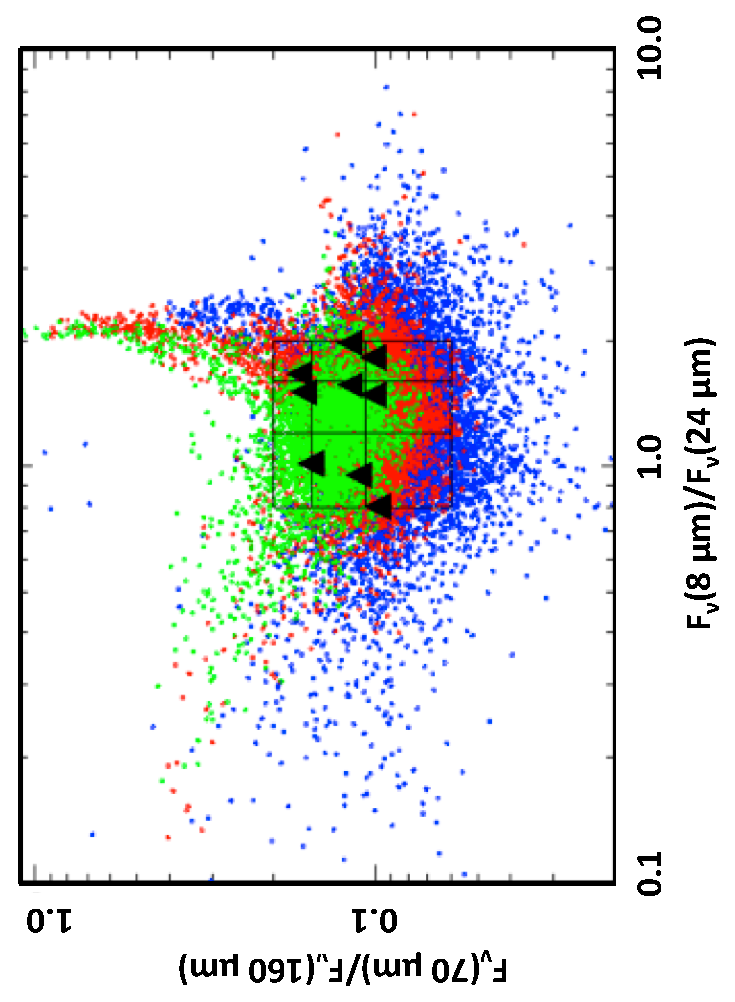
\includegraphics[width = 6.5 cm,angle=270]{fig1.eps}
\caption{$8 - 24/70 - 160$ $\mu$m colour-colour diagram of M31 obtained from IRAC and MIPS imaging. Colour-coding of points represents
24~$\mu$m flux, from faintest (blue) to brightest (red). The plot is divided into 9 regions (black grid), and the observations were made to 
cover those regions subject to a 24~$\mu$m brightness cut. The black triangles indicate colours of the regions we observed.}
\label{colourmaps}
\end{figure}

We obtained mid-infrared spectral maps of 12 regions in M31 using the {\em Spitzer}/IRS instrument \citep{IRS2004} covering wavelengths from 5 to 21 microns. 
A background observation was also made off the galaxy 
along the minor axis for use in background subtraction from the data cubes.
The 12 target regions include the nucleus, the `bulge' and `active' regions previously observed by ISOCAM (the latter is Region 9 in our sample), 
and 9 other regions selected to cover a range of metallicities and dust temperatures.%
\footnote{One additional spectral map in M31 is available in the {\it Spitzer} archive (AOR key 12019200);
unfortunately it does not cover the 5--13~$\mu$m region, which is the major focus of this paper. We therefore elected to not include these observations.} 
These 9 regions were chosen by convolving the IRAC 8~$\mu$m \citep{Barmby2006lr}
and MIPS \citep{gordon06a} maps to the same resolution and constructing an $8 - 24/70 - 160$ $\mu$m colour-colour diagram (Figure~\ref{colourmaps}).
This colour space was used to give a rough definition of the types of spectral energy distribution; the 
dense region in the plot was split into a 3x3 grid and one pixel in each grid region (subject to a 24$\mu$m brightness cut)
was selected for spectroscopy. 
The locations of the observed regions are shown in Figure~\ref{m31}, and 
their coordinates and metallicities are given in Table~\ref{regions}.  
Except for regions 5 and 8, all of our mapped regions contain an  H~{\sc ii} region with
an optical spectroscopic metallicity measurement by \citet{Sanders_2011}; Table ~\ref{regions} gives the measurements from the method 
\citet{Sanders_2011} denote ``N06 N2''  \citep{Nagao2006}. For regions 5 and 8 we estimated metallicities using the M31 radial gradient
that  \citet{Sanders_2011} fit to the H{\sc ii} region ``N06 N2'' measurements: $12+\log{\rm [O/H]} = 9.09 - 0.00195 R{\rm gc}$.

\begin{table*}
 \centering
 \begin{minipage}{90mm}
\caption{Spitzer/IRS Target Locations in M31
\label{regions}}
\begin{tabular}{lccrl}
\hline Name & R.A. (J2000) & Decl. (J2000) & ${R_{\rm gc}}^b$ & $12+\log({\rm O/H})^c$
\\
 \hline
Nucleus$^a$ & $00^{\rmn{h}}42^{\rmn{m}}44\fs31$ & $41\degr16\arcmin09\farcs4$  & 0.0 & \\
Bulge$^a$   & $00^{\rmn{h}}42^{\rmn{m}}35\fs00$ & $41\degr21\arcmin01\farcs0$  & 4.7 &$8.90\pm0.03$\\
Region 1    & $00^{\rmn{h}}41^{\rmn{m}}30\fs41$ & $40\degr43\arcmin07\farcs8$  & 12.4 &$9.20\pm0.20$\\
Region 2    & $00^{\rmn{h}}45^{\rmn{m}}22\fs85$ & $41\degr38\arcmin53\farcs1$  & 13.0 &$9.07\pm0.02$\\
Region 3    & $00^{\rmn{h}}40^{\rmn{m}}37\fs37$ & $41\degr01\arcmin29\farcs4$  & 12.1 &$8.85\pm0.01$\\
Region 4    & $00^{\rmn{h}}41^{\rmn{m}}17\fs86$ & $41\degr07\arcmin09\farcs8$  & 8.7 &$8.89\pm0.06$\\
Region 5    & $00^{\rmn{h}}43^{\rmn{m}}39\fs57$ & $41\degr19\arcmin03\farcs1$  & 7.0 &$8.93\pm0.08$\\
Region 6    & $00^{\rmn{h}}43^{\rmn{m}}35\fs72$ & $41\degr23\arcmin15\farcs0$  & 4.3 &$8.73\pm0.08$\\
Region 7    & $00^{\rmn{h}}40^{\rmn{m}}53\fs98$ & $40\degr58\arcmin58\farcs9$  & 8.7 &$8.40\pm0.08$\\
Region 8    & $00^{\rmn{h}}42^{\rmn{m}}21\fs60$ & $41\degr07\arcmin17\farcs4$  & 3.1 &$8.94\pm0.08$\\
Region 9$^a$& $00^{\rmn{h}}41^{\rmn{m}}00\fs00$ & $40\degr36\arcmin20\farcs3$  & 13.5 &$8.86\pm0.02$\\
NGC~206     & $00^{\rmn{h}}40^{\rmn{m}}20\fs20$ & $40\degr44\arcmin54\farcs0$  & 9.8 & \\
Background  & $00^{\rmn{h}}44^{\rmn{m}}41\fs80 $ & $40\degr58\arcmin56\farcs0$  & 29.5 & \\
\hline
\end{tabular}
{$^a$Regions with ISOCAM data.\\
$^b$De-projected galactocentric distance in kpc.\\ 
$^c$Metallicities from \citet{Sanders_2011}, except for Regions 5 and 8 where metallicities are estimated from the radial metallicity profile.
}
\end{minipage}
\end{table*}

\begin{figure*}
\centering
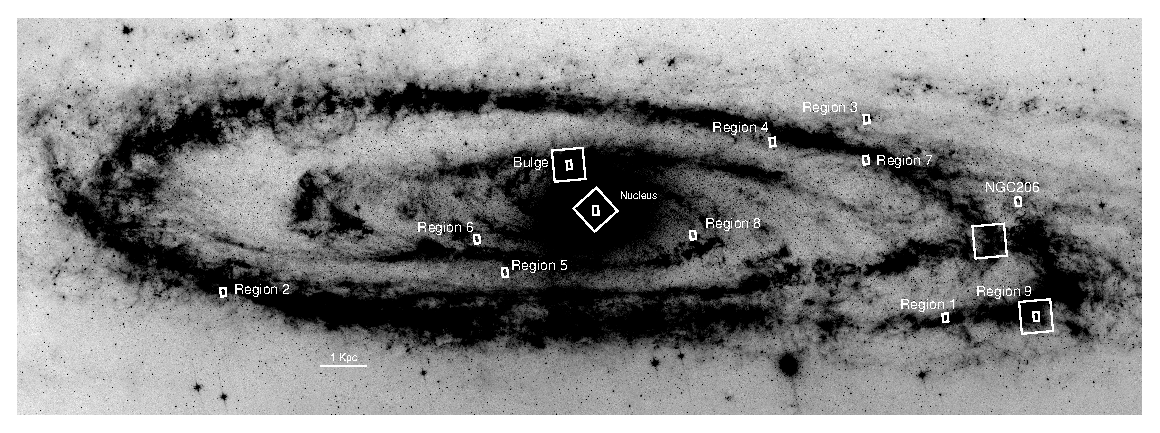
\includegraphics[scale=0.9]{./fig2.eps}
\caption{An 8 micron negative IRAC image of M31 \citep{Barmby2006lr}. Small white rectangles ($30\arcsec\times50\arcsec$) show the regions that we observed, and larger squares ($192\arcsec\times192\arcsec$) show the regions observed by  \citet{1998Cesarsky}.
\label{m31}
}
\end{figure*}


For our observations we used the IRS Short-Low (SL) and Long-Low (LL) modules, which cover wavelengths from 5 to 21 microns. 
The Low modules have resolving power in the range 60--130. Each low-resolution module is divided into two sub-slits 
which provide spectroscopy in either first or second order. They are denoted as SL1 (7.5--14.5~$\mu$m), SL2 (5.2--7.6~$\mu$m),
LL1 (20.5--38.5~$\mu$m, not used in these observations), and LL2 (14.5--20.75~$\mu$m).
All M31 regions were observed in September 2007 as part of G. G. Fazio's Guaranteed Time (program ID 40032). 
The map size was based on the size 
of the IRS slits (SL: $3.6\arcsec \times 57\arcsec$, LL: $10.5\arcsec \times 168\arcsec$). Each region was covered by 18 overlapping observations 
of the SL slit and 11 overlapping observations of the LL slit making the map size $32\arcsec \times 57\arcsec$ for SL and $58\arcsec \times 168\arcsec$ for LL. 
Figure~\ref{slits} shows an example of the slit arrangement. For the brighter regions (nucleus, bulge), ramp times of 14 s (SL) and 30 s (LL) were used, 
while for the fainter regions, ramp times of 60 and 120 s were used respectively. Background observations were taken with each module (2 per ramp time). 
Because all of the targets are in the same part of the sky, a common background observation was used for multiple targets to subtract the background emission. 

\begin{figure}
\centering
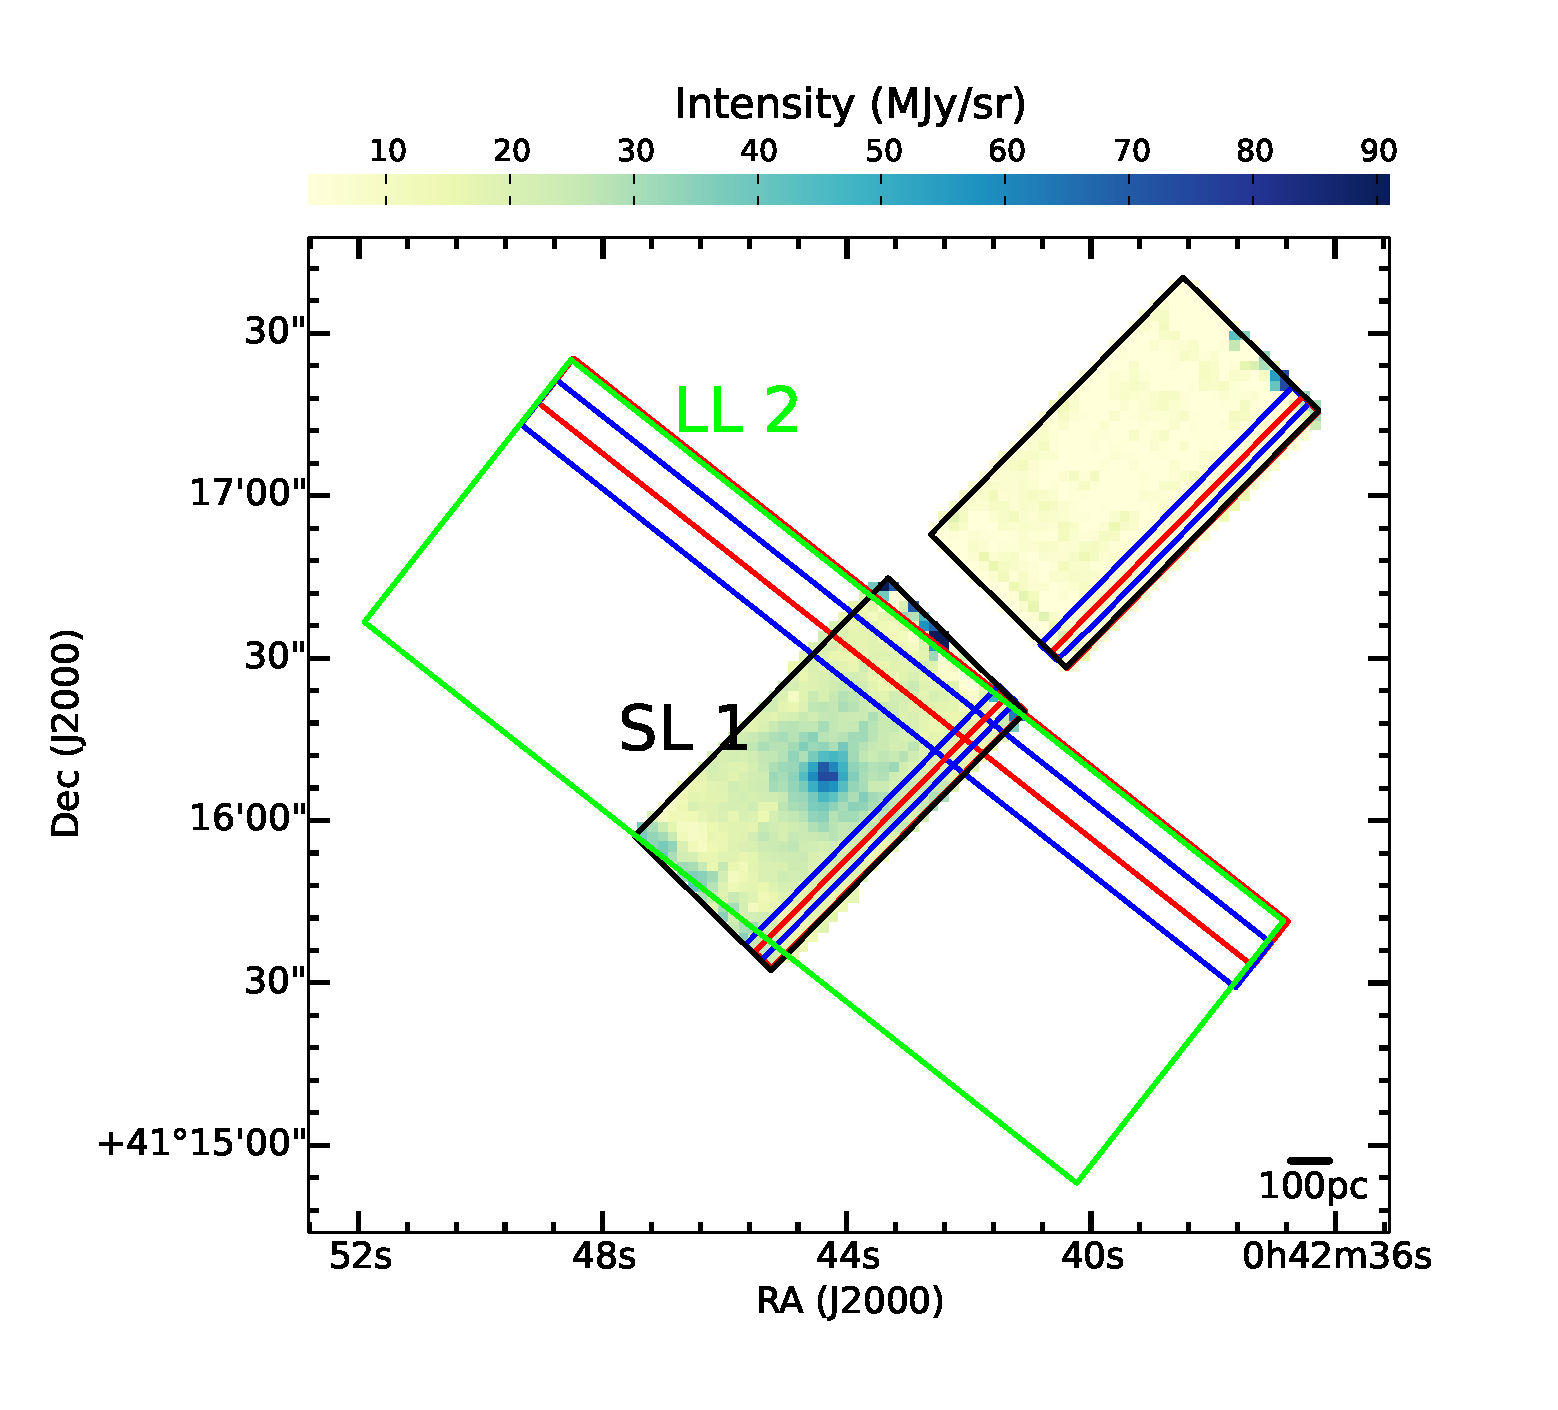
\includegraphics[scale=0.3]{./fig3.eps}
\caption{The 7.6~$\mu$m plane constructed from the SL1 data cube of the nucleus, showing the arrangement of slits used to cover the region. 
Black boxes outline the footprint of the SL1 maps (the off-center SL1 map is from observations made
when SL2 was centred) and the green box outlines the LL2 map. 
Blue and red slits show how  each map was covered using overlapping slit positions.
\label{slits}
}
\end{figure}

\subsection{IRS Data Reduction}
\label{sect:irs_data}

The data were reduced through the SSC pipeline (ver. S17.2.0), and the maps were assembled using the CUBISM program \citep{Smith:2007fk}. 
Bad pixel removal was also done using CUBISM, and the background observations were used to subtract the background emission from these cubes 
following the method outlined by \citet{Gordon:2008lr}. Spectra were extracted using a $30\arcsec\times50\arcsec$   rectangular aperture,
which corresponds to $114\times190$~pc at the distance of M31.
The aperture size was selected to cover the overlapping area of the SL and LL modes; all the IRS maps cover more area than  considered here.
In order to study the spatial variation of the emission near the nucleus, we also extracted spectra from two smaller regions
within that map; these will be further discussed in Section~\ref{sect:nucleus}.
The spectrum of NGC 206 is very noisy and was removed from our analysis. 

% REF:
%Section 2.2:
%Why did you not include the bonus order (SL3) data to help in the overlap regions of the SL matching?
%
%There is a synthetic IRAC 4 tool inside CUBISM which takes the spectral cube and produces a map as it would be observed through the IRAC 4 filter. Comparing this map with the map from Barmby et al 2006 and deriving a correction factor seems to be more straight-forward than the method you describe.
%
%I did not understand ***why*** the SL and LL orders do not match naturally and instead have a systematic offset. Also the calculated offset (table 2) is positively correlated with the IRAC 4 photometry, why?
%
%The statement about the non-zero intercept and thus opting to apply an offset correcting is unconvincing given that you find an offset compatible with 0 (-0.05 +- 0.06) and a slope which is significantly different than unity.


There is wavelength overlap between the SL1 and SL2 spectra and also between the SL1 and LL2 spectra.
To generate a single spectrum for each M31 region it is necessary to combine the spectra and
account for photometric offsets between them. Such offsets are commonly seen in IRS spectra extracted
from extended regions, since the slit loss is not well-characterized (**Els please check this sentence**).
The SL1 and SL2 flux densities were
generally quite well-matched over the wavelength overlap region ($7.5 < \lambda< 7.6\mu$m)
and those two orders were combined by averaging fluxes over the  overlap region.
In cases with offsets between SL1 and SL2, we found that SL2 and the `bonus order' SL3 were well-matched.
We  combined the  SL1 and SL3 
spectra by computing the average flux densities over the  overlap region and
adding a constant  to the SL1 spectra so that they matched the SL3 average. The SL1 and SL2 orders
were then combined as described above.
After this procedure there was still a noticeable mis-match between the SL and LL spectra. We addressed this
by scaling the SL spectra to match IRAC 8~$\mu$m fluxes as follows. IRAC fluxes were measured
on the 8~$\mu$m image \citep{Barmby2006lr} in the same apertures used to extract the IRS spectra.
An extended source  aperture correction of 0.824 was applied to the IRAC fluxes; this value was computed 
using the formula in the IRAC Data Handbook \citep{} with
the radius of a circular aperture having the same area as the extraction aperture.
The {\em Spitzer} synthetic photometry software \citep{SpitzerDAC} 
was then used to quantify the colour correction for each spectrum, i.e. the
multiplicative factor $K$ between the IRAC photometry over its broad bandpass and the IRS flux
density at the centre of the bandpass.  For each spectrum we computed the additive
offset between the color-corrected IRS flux density and the IRAC aperture-corrected flux density,
and used this to correct the SL spectra; this method was also used by \citet{Sandstrom12}.
Although a multiplicative offset could also have been used to match the IRS photometry to IRAC,
the resulting change in spectral slope increased the size of the SL/LL offset.
The SL spectra corrected with additive offsets were closely-matched to the LL spectra, and the final combination
of SL and LL was done using the average-and-offset procedure described above for SL1 and SL3.



\subsection{ISOCAM Data Reduction}
\label{sect:iso_data}

To compare our results with those of  \citet{1998Cesarsky}, we retrieved the highly processed ISOCAM data provided by \citet{Boulanger_F_2005}  
for the nucleus, bulge, and region 9. 
The ISOCAM data were obtained with the circular variable filters (CVFs) over a $3\arcmin \times 3\arcmin$ field of view at a scale of 6\arcsec\ per pixel. 
The wavelength range covered was 5.15--16.5~$\mu$m at a resolution of $\lambda/\Delta \lambda \approx 45$; the ISOCAM instrument is described by \citet{cesarsky1996}.
An example image of the ISOCAM data is shown in Figure~\ref{isonuc}.  For the three regions, we extracted spectra using the same 
$30\arcsec\times50\arcsec$ aperture as for the IRS data. 

\begin{figure}
\centering
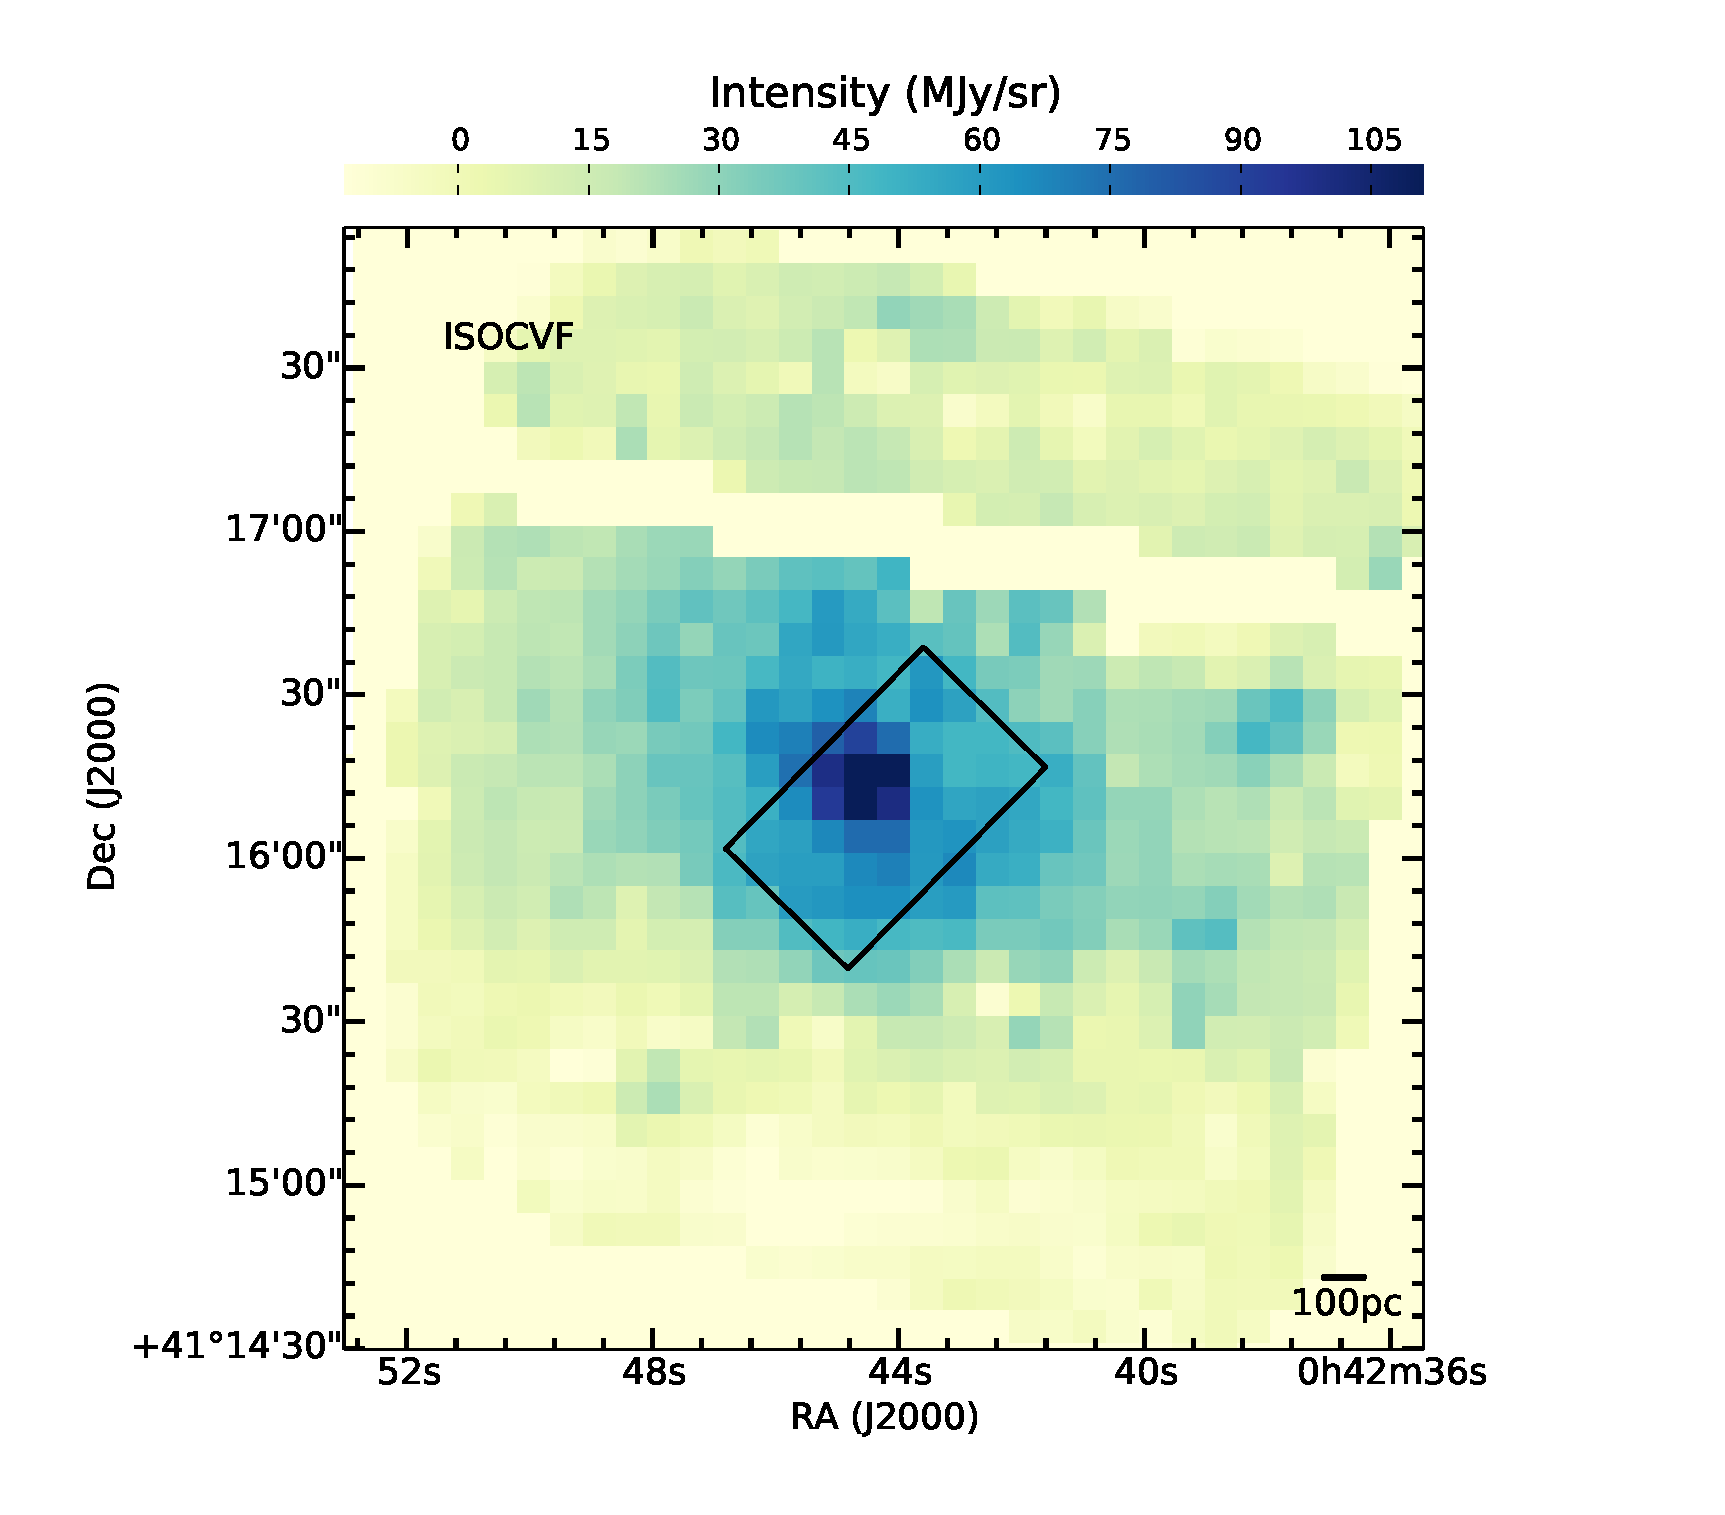
\includegraphics[width = 8cm]{./fig4.eps}
\caption{11.3~$\mu$m negative image (dark colours indicate higher flux) of the ISOCAM data cube from the nucleus of M31. 
The black box shows the size of the aperture ($30\arcsec\times50\arcsec$) used to extract spectra.}
\label{isonuc}
\end{figure}







% MLNA: The title of Sec 3 should be more specific; data analysis sounds akin to data reduction.  
\section{Data analysis}
\label{sect:data_analysis}

%REF:
%Section 3:
%How reliable are the uncertainties in table 3? Some uncertainties seem small to me. It is also surprising to see how constant these uncertainties are in absolute value from region to region for a quite variable set of input spectra. As one example: it does not make much sense to me that the absolute uncertainty on the 6.2 band in region #1 and region #8 are identical. The uncertainties on the smaller bands like the 12.0 um band are small (e.g. region 9 or the bulge). You yourself (implicitly) cast a doubt on the uncertainties when you discuss the outliers in figure 12 (sect 4.3).

The final processed IRS spectra are shown in  Figure \ref{PAHFITplots}, except for the nucleus, discussed in Section~\ref{sect:nucleus}.
All of the main PAH features, including the 6.2, 7.7, 8.6 and 11.3~$\mu$m bands, 
are clearly visible for all the regions shown here.
The IRS spectra also show atomic line emission such as [Ar~{\sc ii}], [Ar~{\sc iii}], [S~{\sc iii}], [S~{\sc iv}], [Ne~{\sc ii}], [Ne~{\sc iii}] 
and molecular H$_{2}$ emission at 12.3~$\mu$m. Some of the spectra display a contribution to the continuum from starlight emission.


\begin{figure*}
\centering
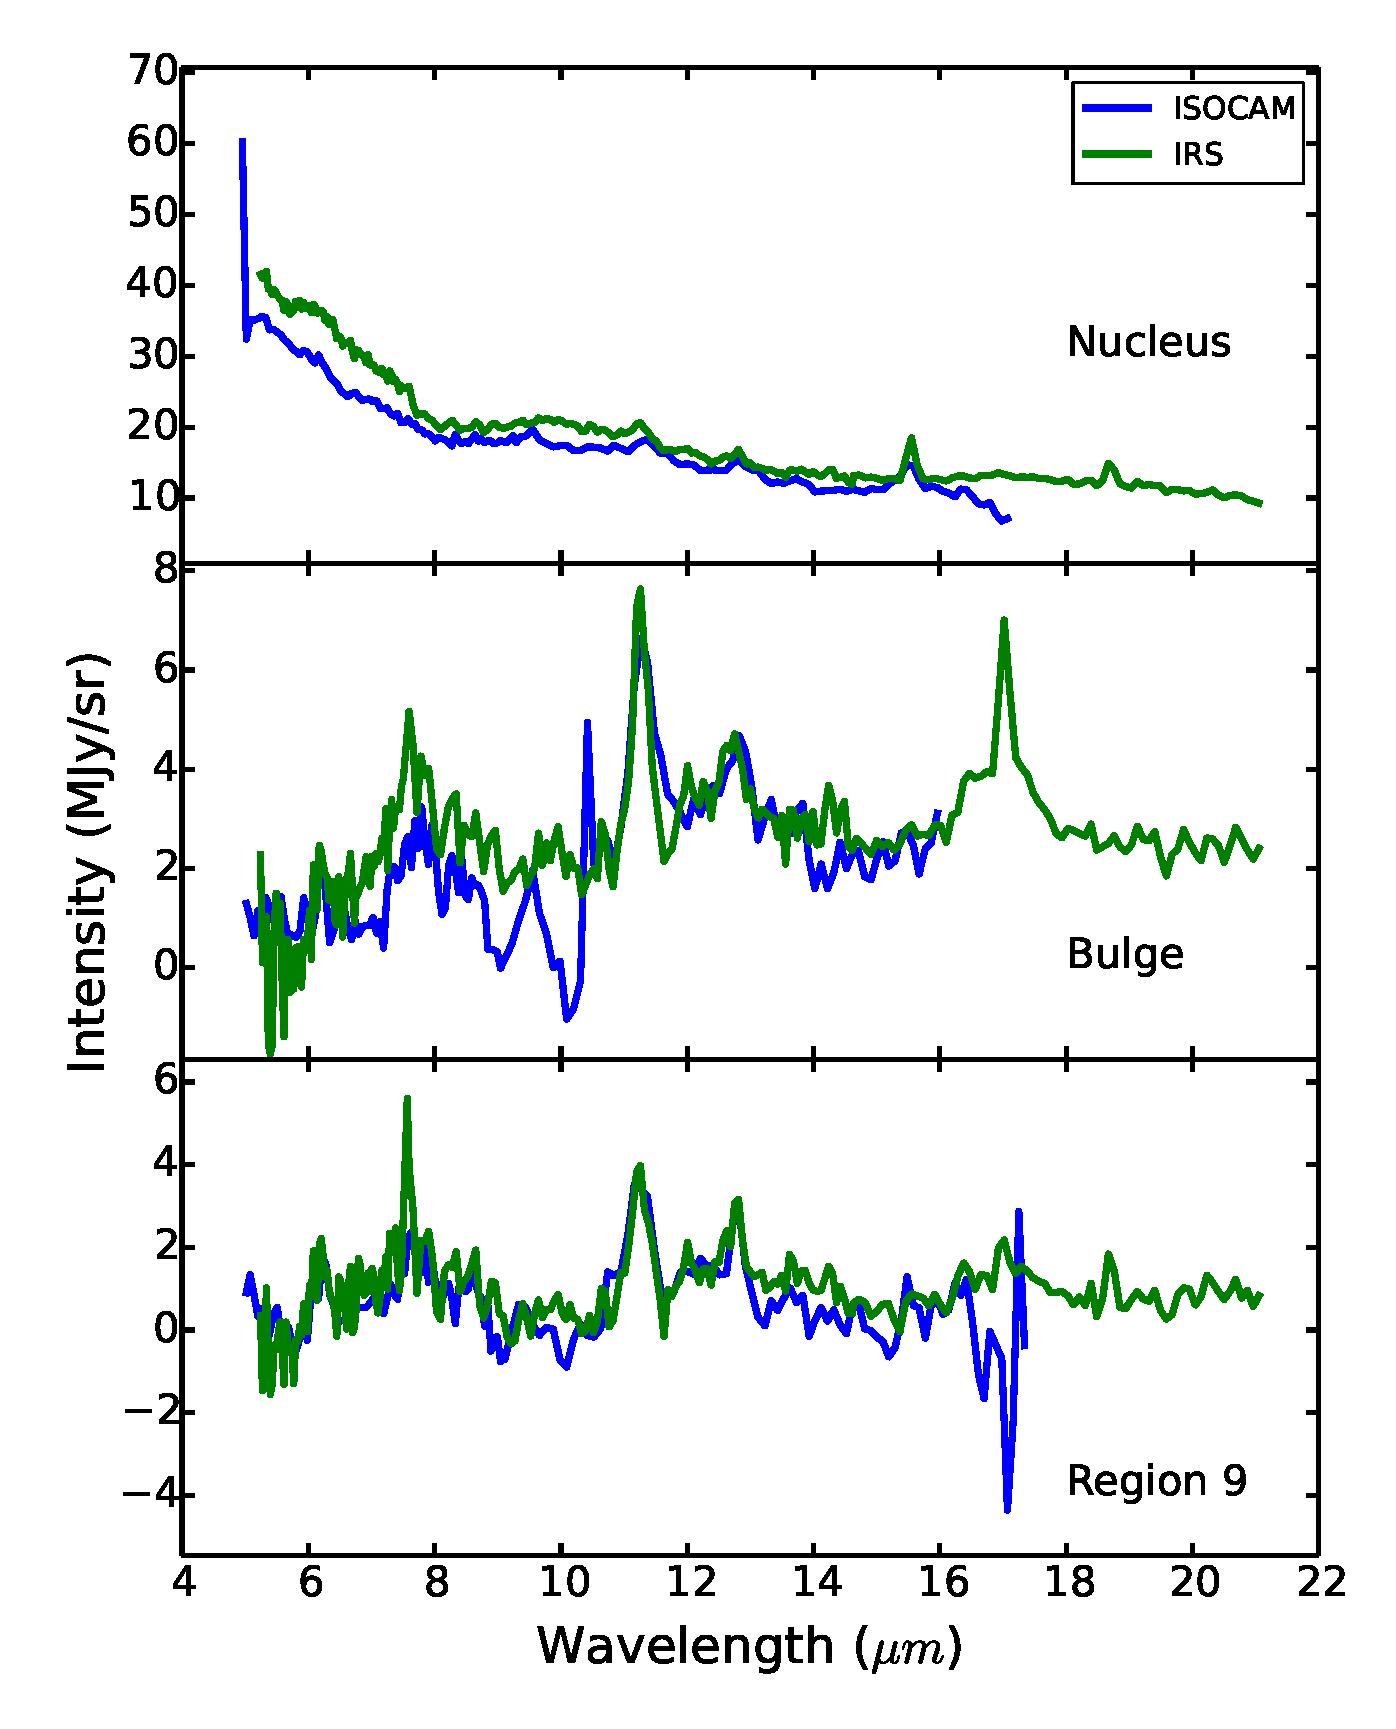
\includegraphics[scale=0.45]{./fig6.eps}
 \caption{Observed IRS spectra and detailed PAHFIT decompositions (see Section~\ref{sect:pahfit}). Regions are labeled in each panel.
Black squares show the observed data, and red, blue, light blue, pink and green lines represent the modelled
dust continua, PAH features, atomic lines, starlight continuum and the fit respectively. The black line shows the total modelled continuum. 
Vertical scales differ in different panels. Spectra from the nucleus and NGC 206 are not shown here.
}
\label{PAHFITplots}
\end{figure*}


\subsection{ISOCAM versus IRS}
\label{sect:iso_vs_irs}

As mentioned in the Introduction, based on ISOCAM observations of four regions in M31, \citet{1998Cesarsky} reported 
suppression of the common 6--8~$\mu$m PAH bands and a strong 11.3$\mu$m PAH band.
The 11.3~$\mu$m band profile was found to vary from region to region.  
In addition, \citet{Pagani_1999} confirmed that the star-forming ring in M31 shows very weak PAH emission in the 6 to 8~$\mu$m region. 
However, the IRS spectra presented here, except the nucleus, do not show such unusual behaviour (Figure~\ref{PAHFITplots}). 
Indeed all regions, except the nucleus, show a normal mid-infrared spectrum similar to other nearby starforming galaxies. 

Until 2005, ISOCAM-CVF data were not properly background subtracted and they were contaminated with zodiacal emission and stray light. 
Differential spectra between regions of relatively strong and weak emission were previously used to overcome this problem 
(more details about the differential spectra are given by \citealt{1998Cesarsky}, \citealt{Pagani_1999}). 
In 2005, all ISOCAM-CVF data were reprocessed  and corrected for the zodiacal emission \citep{Boulanger_F_2005}. 
We obtained newly-processed ISOCAM spectra from three regions in our IRS sample (see Section~\ref{sect:iso_data}) 
in order to compare them with the corresponding IRS spectra.
Figure~\ref{ISOnIRS} shows that although the relative feature intensities  in the IRS and ISOCAM 
spectra differ in detail, the spectral shapes are almost identical;
the re-processed ISOCAM data do not agree with the previous differential spectra.
Neither the bulge nor Region 9 shows any depletion in  6 to 8~$\mu$m features as described by \citet{1998Cesarsky}. 
The new ISOCAM reduction appears to eliminate the discrepancies between ISOCAM and IRS, resulting
in less `strange' infrared spectra for M31. For the remainder of this work, we discuss only the IRS spectra.



\begin{figure}
\centering
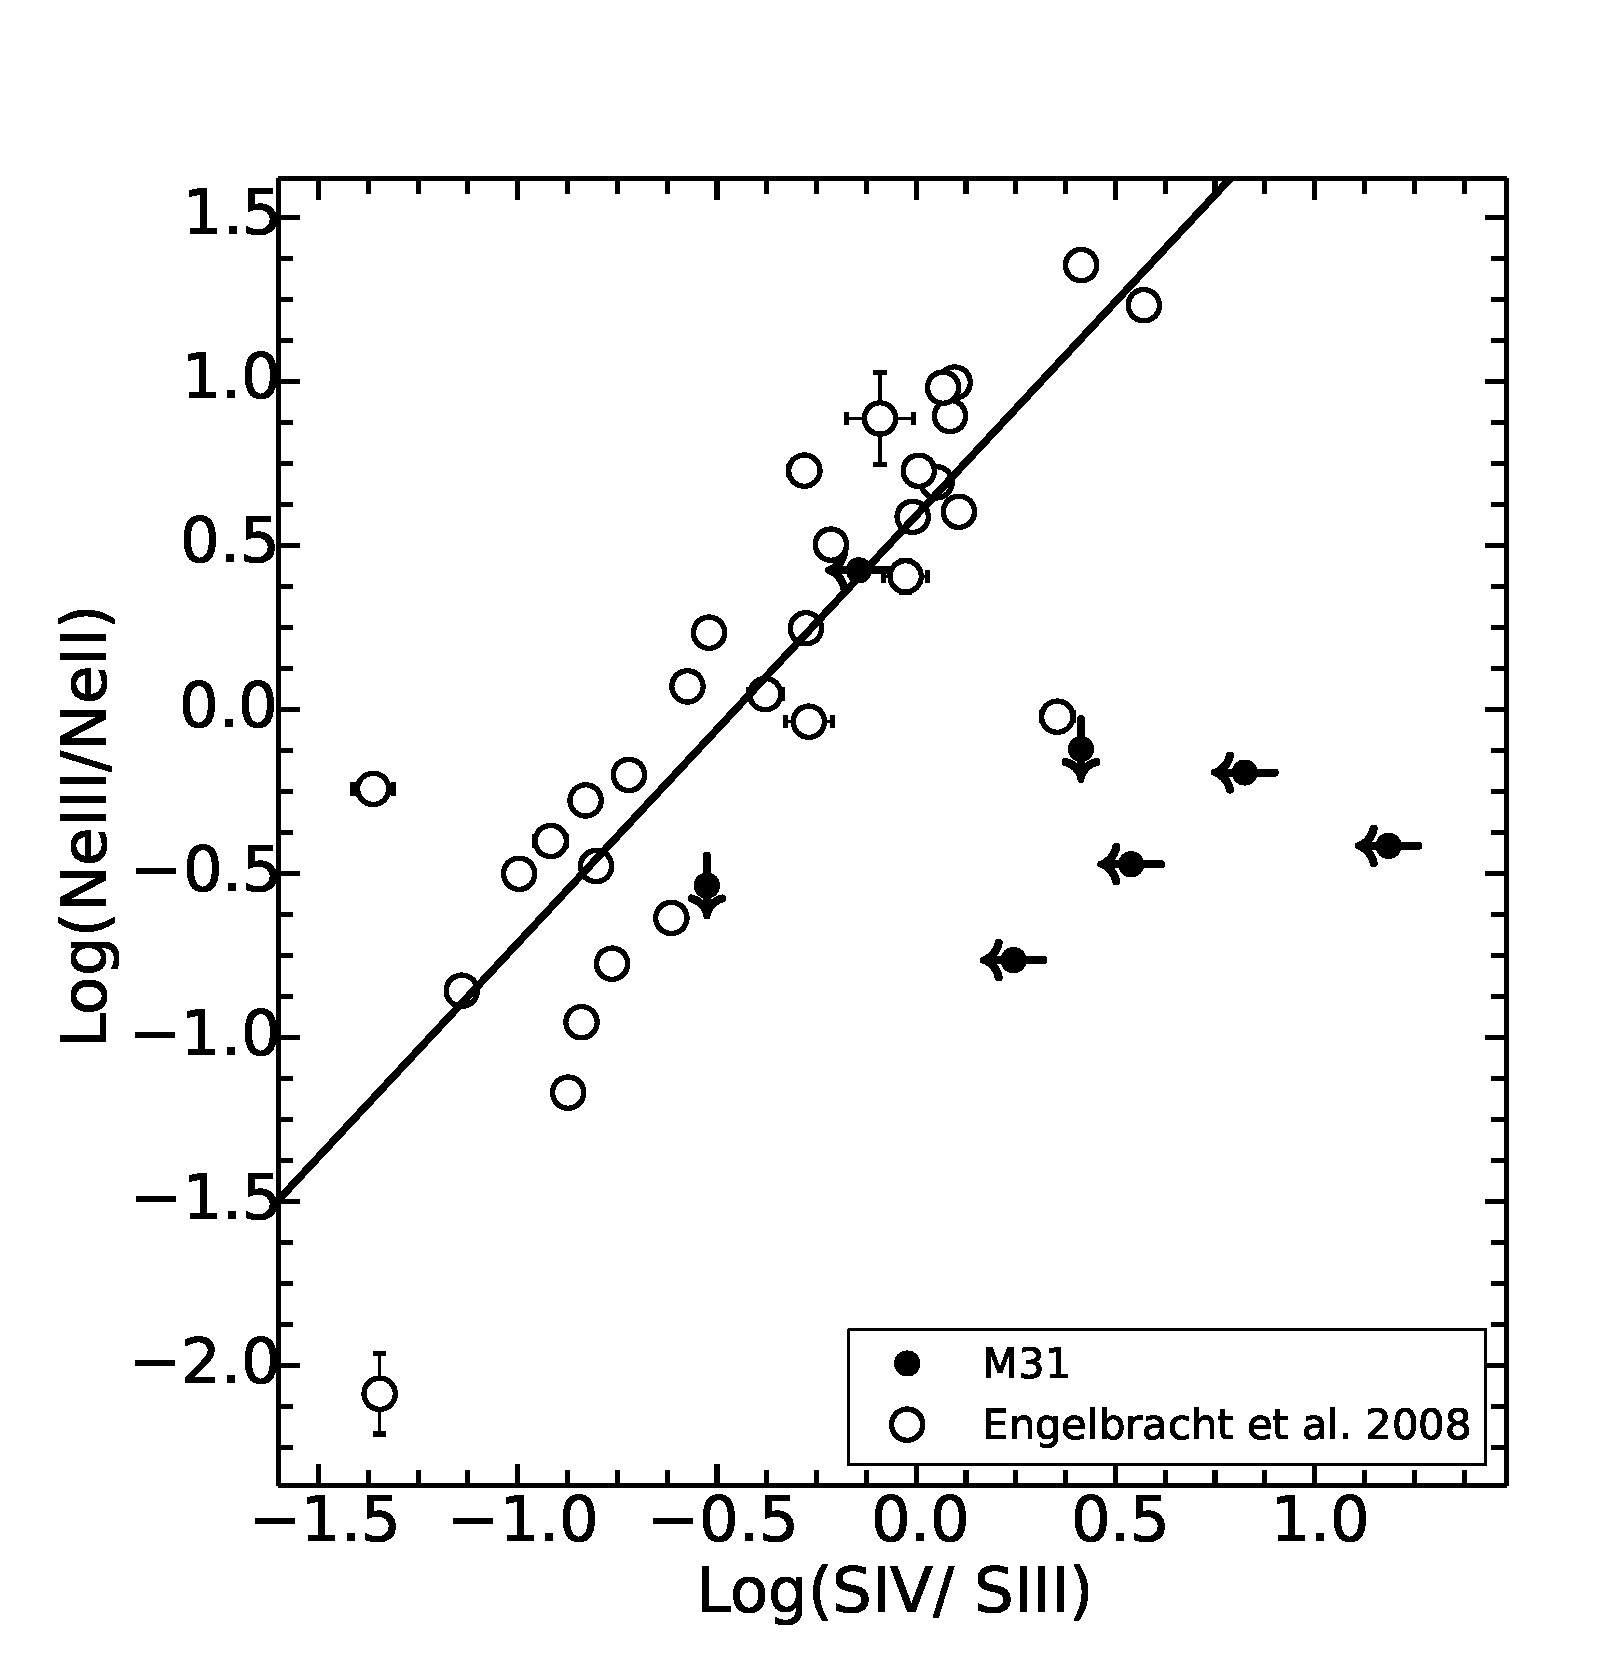
\includegraphics[scale=0.35]{./fig7.eps}
\caption{ Comparison of  IRS and re-processed ISOCAM spectra for the Nucleus (top), Bulge (middle) and Region 9 (bottom) in M31.}
\label{ISOnIRS}
\end{figure}



\subsection{PAHFIT}
\label{sect:pahfit}
The PAH features in  IRS spectra are often blended with neighbouring PAH features and atomic lines. 
Therefore measuring the strength of PAH features is difficult.  To achieve this task a tool called PAHFIT, introduced by \citet{Smith:2007lr}, was used. 
PAHFIT is an IDL  based tool designed for decomposing {\em Spitzer} IRS low-resolution spectra of PAH emission sources.
PAHFIT uses six main components to fit the surface brightness. These are starlight continuum, featureless thermal dust continuum, 
pure rotational lines of H$_2$, fine-structure lines, dust emission features and dust extinction. The starlight is represented by  blackbody 
emission at a fixed temperature of 5000~K, and the dust continuum is represented by 8 modified blackbodies (emissivity proportional to $\nu^2$)  
at fixed temperatures of 35, 40, 50, 65, 90, 135, 200, and 300~K. The final fit obtained with PAHFIT does not necessarily use
all eight dust components.
The infrared extinction is considered as a combination of a power law plus silicate absorption features with peaks at 9.7 and 18~$\mu$m. 
Line features are represented by Gaussian profiles with widths set by the instrumental resolution
and dust features are represented by Drude profiles; more details about PAHFIT are given by \citet{Smith:2007lr}.


Initial attempts at fitting the spectra with PAHFIT showed that some components were negligible, and
to avoid over-fitting we re-ran the fits without these components.
None of the IRS spectra shows significant silicate absorption around 9.7 or 18~$\mu$m, and the extinction calculated by PAHFIT 
was almost zero for all the initial fits. Except for four regions (the bulge, Region 5, Region 6 and Region 8),
the starlight contribution is also negligible.
We adjusted the PAHFIT input parameters to fix extinction to zero for all regions and starlight to zero for all but the four regions above.
Typically only two or three thermal dust components had significant power in our fits, but we did not fix the unused components to zero.
Regions 3 and 9 were found to have very low dust continuum emission compared to other spectra,
possibly because of noisy data at short wavelengths. However the other features in these spectra appear to
be fit correctly. The spectrum of the nucleus shows silicate emission, which is not included in PAHFIT;  
our modifications of PAHFIT to analyze this spectrum are discussed in see Section~\ref{sect:nucleus}.

\begin{table*}
 \centering
 \begin{minipage}{200mm}
\caption{PAH Emission Line Strengths$^a$}
{\scriptsize
  \begin{tabular}{l c c  c  c  c  c  c  c  c  c c }
\hline
    {Region }&{5.7 $\mu$m  }&{6.2 $\mu$m  }&{7.7 $\mu$m$^b$  }&{8.3 $\mu$m  }&{8.6 $\mu$m  }&{10.7 $\mu$m  }&{11.3 $\mu$m$^b$  }&{12.0 $\mu$m  }&{12.7 $\mu$m$^b$  }&{17.0 $\mu$m$^b$  } \\
 \hline
  %  Pub_ID  PAH5.7flx  PAH6.2flx  PAH7.7flx  PAH8.3flx  PAH8.6flx  PAH10.7flx  PAH11.3flx  PAH12.0flx  PAH12.7flx  PAH17.0flx 
%  None  1e-15W/m2  1e-15W/m2  1e-15W/m2  1e-15W/m2  1e-15W/m2  1e-15W/m2  1e-15W/m2  1e-15W/m2  1e-15W/m2  1e-15W/m2 
       Bulge  & \dots & $1.32 \pm 0.08$ & $7.7 \pm 0.6$ & $1.1 \pm 0.2$ & $0.7 \pm 0.1$ & $0.07 \pm 0.03$ & $1.85 \pm 0.08$ & $0.49 \pm 0.05$ & $1.02 \pm 0.09$ & $1.39 \pm 0.04$\\
    Region 1  & $0.36 \pm 0.05$ & $1.20 \pm 0.04$ & $3.8 \pm 0.2$ & $0.46 \pm 0.04$ & $0.50 \pm 0.03$ & $0.08 \pm 0.01$ & $1.18 \pm 0.02$ & $0.32 \pm 0.02$ & $0.54 \pm 0.02$ & $0.58 \pm 0.02$\\
    Region 2  & $0.27 \pm 0.03$ & $1.10 \pm 0.03$ & $3.7 \pm 0.2$ & $0.33 \pm 0.04$ & $0.70 \pm 0.03$ & $0.053 \pm 0.008$ & $1.13 \pm 0.02$ & $0.23 \pm 0.01$ & $0.51 \pm 0.03$ & $0.51 \pm 0.02$\\
    Region 3  & $0.3 \pm 0.1$ & $0.9 \pm 0.1$ & $3.9 \pm 0.6$ & $0.7 \pm 0.1$ & $0.3 \pm 0.1$ & \dots & $0.68 \pm 0.07$ & $0.21 \pm 0.05$ & $0.47 \pm 0.07$ & $0.45 \pm 0.04$\\
    Region 4  & $0.14 \pm 0.04$ & $0.56 \pm 0.03$ & $2.1 \pm 0.2$ & $0.26 \pm 0.04$ & $0.41 \pm 0.03$ & $0.029 \pm 0.008$ & $0.70 \pm 0.02$ & $0.12 \pm 0.01$ & $0.31 \pm 0.02$ & $0.44 \pm 0.02$\\
    Region 5  & \dots & $0.24 \pm 0.04$ & $0.79 \pm 0.07$ & $0.12 \pm 0.04$ & $0.21 \pm 0.03$ & $0.032 \pm 0.008$ & $0.45 \pm 0.02$ & $0.09 \pm 0.01$ & $0.22 \pm 0.01$ & $0.33 \pm 0.04$\\
    Region 6  & \dots & $0.26 \pm 0.03$ & $0.8 \pm 0.2$ & $0.10 \pm 0.03$ & $0.13 \pm 0.03$ & $0.029 \pm 0.008$ & $0.38 \pm 0.02$ & $0.07 \pm 0.01$ & $0.16 \pm 0.01$ & $0.29 \pm 0.02$\\
    Region 7  & $0.21 \pm 0.03$ & $0.62 \pm 0.03$ & $2.0 \pm 0.2$ & $0.30 \pm 0.04$ & $0.45 \pm 0.03$ & $0.058 \pm 0.008$ & $0.77 \pm 0.02$ & $0.18 \pm 0.01$ & $0.37 \pm 0.03$ & $0.47 \pm 0.04$\\
    Region 8  & \dots & $0.09 \pm 0.04$ & $0.22 \pm 0.07$ & $0.09 \pm 0.04$ & $0.10 \pm 0.03$ & $0.051 \pm 0.009$ & $0.16 \pm 0.02$ & \dots & \dots & $0.15 \pm 0.02$\\
    Region 9  & \dots & $1.3 \pm 0.1$ & $4.4 \pm 0.6$ & $0.9 \pm 0.1$ & $0.5 \pm 0.1$ & $0.09 \pm 0.03$ & $1.32 \pm 0.07$ & $0.51 \pm 0.05$ & $0.83 \pm 0.07$ & $0.6 \pm 0.1$\\

 \hline
 \label{PAHlinetable}
\end{tabular}\\
{$^a$Units are 10$^{-15}$~W~m$^{-2}$.\\
$^b$PAH complexes, as described in text.}
}
\end{minipage}
\end{table*}



\begin{table*}
 \centering
 \begin{minipage}{200mm}
 
\caption{PAH Emission Line Equivalent Widths$^a$}
 {\scriptsize
  \begin{tabular}{l c c  c  c  c  c  c  c  c  c c }
  \hline 
     {Region }&{5.7 $\mu$m  }&{6.2 $\mu$m  }&{7.7 $\mu$m$^b$  }&{8.3 $\mu$m  }&{8.6 $\mu$m  }&{10.7 $\mu$m  }&{11.3 $\mu$m$^b$  }&{12.0 $\mu$m  }&{12.7 $\mu$m$^b$  }&{17.0 $\mu$m$^b$  } \\
 \hline
 %  Pub_ID  PAH5.7eqw  PAH6.2eqw  PAH7.7eqw  PAH8.3eqw  PAH8.6eqw  PAH10.7eqw  PAH11.3eqw  PAH12.0eqw  PAH12.7eqw  PAH17.0eqw 
%  None  micron  micron  micron  micron  micron  micron  micron  micron  micron  micron 
       Bulge  & \dots & $1.2 \pm 0.2$ & $4.1 \pm 0.4$ & $0.51 \pm 0.07$ & $0.30 \pm 0.06$ & $0.03 \pm 0.01$ & $0.78 \pm 0.04$ & $0.22 \pm 0.02$ & $0.49 \pm 0.05$ & $1.16 \pm 0.04$\\
    Region 1  & $0.39 \pm 0.08$ & $1.2 \pm 0.1$ & $3.4 \pm 0.3$ & $0.43 \pm 0.04$ & $0.47 \pm 0.04$ & $0.09 \pm 0.01$ & $1.45 \pm 0.04$ & $0.43 \pm 0.03$ & $0.76 \pm 0.04$ & $1.26 \pm 0.05$\\
    Region 2  & $0.28 \pm 0.04$ & $1.02 \pm 0.06$ & $3.4 \pm 0.2$ & $0.32 \pm 0.04$ & $0.70 \pm 0.04$ & $0.07 \pm 0.01$ & $1.58 \pm 0.04$ & $0.35 \pm 0.02$ & $0.85 \pm 0.05$ & $1.33 \pm 0.06$\\
    Region 3  & $4.3 \pm 2.3$ & $8.3 \pm 2.3$ & $18.5 \pm 4.2$ & $2.8 \pm 0.8$ & $0.9 \pm 0.5$ & \dots & $2.1 \pm 0.3$ & $0.7 \pm 0.2$ & $1.6 \pm 0.3$ & $2.4 \pm 0.3$\\
    Region 4  & $0.28 \pm 0.09$ & $1.0 \pm 0.1$ & $3.7 \pm 0.4$ & $0.48 \pm 0.07$ & $0.77 \pm 0.07$ & $0.07 \pm 0.02$ & $1.67 \pm 0.06$ & $0.31 \pm 0.04$ & $0.82 \pm 0.06$ & $1.65 \pm 0.08$\\
    Region 5  & \dots & $0.12 \pm 0.03$ & $0.61 \pm 0.07$ & $0.10 \pm 0.03$ & $0.20 \pm 0.03$ & $0.05 \pm 0.01$ & $0.77 \pm 0.04$ & $0.17 \pm 0.03$ & $0.50 \pm 0.04$ & $1.6 \pm 0.2$\\
    Region 6  & \dots & $0.10 \pm 0.04$ & $0.6 \pm 0.2$ & $0.10 \pm 0.04$ & $0.14 \pm 0.03$ & $0.05 \pm 0.01$ & $0.77 \pm 0.05$ & $0.15 \pm 0.03$ & $0.42 \pm 0.05$ & $1.7 \pm 0.1$\\
    Region 7  & $0.32 \pm 0.05$ & $0.86 \pm 0.06$ & $2.2 \pm 0.1$ & $0.44 \pm 0.06$ & $0.69 \pm 0.06$ & $0.12 \pm 0.02$ & $1.81 \pm 0.07$ & $0.48 \pm 0.05$ & $1.08 \pm 0.09$ & $2.2 \pm 0.3$\\
    Region 8  & \dots & \dots & $0.10 \pm 0.05$ & $0.09 \pm 0.04$ & $0.10 \pm 0.03$ & $0.09 \pm 0.02$ & $0.30 \pm 0.04$ & \dots & \dots & $0.62 \pm 0.08$\\
    Region 9  & \dots & $\left(2.4 \pm 1.1\right) \times 10^{2}$ & $\left(1.4 \pm 0.4\right) \times 10^{2}$ & $15.5 \pm 5.6$ & $7.9 \pm 2.8$ & $0.5 \pm 0.2$ & $6.8 \pm 1.1$ & $2.3 \pm 0.6$ & $3.5 \pm 0.8$ & $2.2 \pm 0.8$\\

 \hline
 \label{EQW}
\end{tabular}\\
{$^a$Units are $\mu$m.\\
$^b$PAH complexes, as described in text.\\
Continuum for Regions 3 and 9 is very weak.  Equivalent widths are highly uncertain and not considered in the analysis (see Section~\ref{sect:data_analysis}).}
}
\end{minipage}
\end{table*}



\subsection{PAH features}
\label{sect:pah}

PAHFIT returns fluxes and equivalent widths (EQWs) of PAH features, which are given in Tables~\ref{PAHlinetable} and \ref{EQW}. 
For easier comparison with previous work, the tables give measurements for the 7.7, 11.3, 12.7 and 17.0~$\mu$m PAH complexes
as defined by \citet{Smith:2007lr}, as computed from the individual constituent features measured by PAHFIT.
The intensities of the features do not include any contribution from the continuum, but the equivalent width computed by
\begin{equation}
{\rm EQW}=\int \frac{I_{\nu,{\rm feature}}}{I_{\nu, {\rm cont}}} \,d\lambda,
\end{equation}
is a measure of the ratio of the continuum emission ($I_{\nu, {\rm cont}} $) to the line strength 
($I_{\nu,{\rm feature}}=I_{\nu} =- I_{\nu, {\rm cont}})$. 
The continuum emission is mainly from dust grains, much larger than PAH molecules. Hence, by studying EQWs of PAHs, 
we can study how the PAHs compete with the dust grains in the mid-infrared wavelengths.  PAHFIT returns the EQWs for each PAH 
feature, we calculated the uncertainties using a Monte-Carlo method. In that method, for each region, PAHFIT was run 500 times on 
randomly generated data points  normally distributed within the uncertainties of the spectrum. PAHFIT returned 500 EQWs for each 
PAH feature, and the standard deviation of EQWs for a given feature was taken as its uncertainty. 
The EQWs from Regions 3 and 9 were removed from further analysis because the negligible dust continuum for these spectra makes
the EQWs highly uncertain.


\subsection{Atomic line features}
\label{sect:atomic}

% REF
%Sect 3.4:
%It is not true that keeping only one term of this equation gives you the same RHI as the full equation. The appropriate thing to do; under the assumption that the RHI from Chad Engelbracht paper is applicable to your regions; is to project the points in figure 8 on the straight line and attribute the corresponding value from equation 3. Take for example the right most open dot which is very close to the line. If I calculate RHI using term 1, 2 or both together I find 1.2, 1.42 and 1.31, respectively.

\begin{figure}
\centering
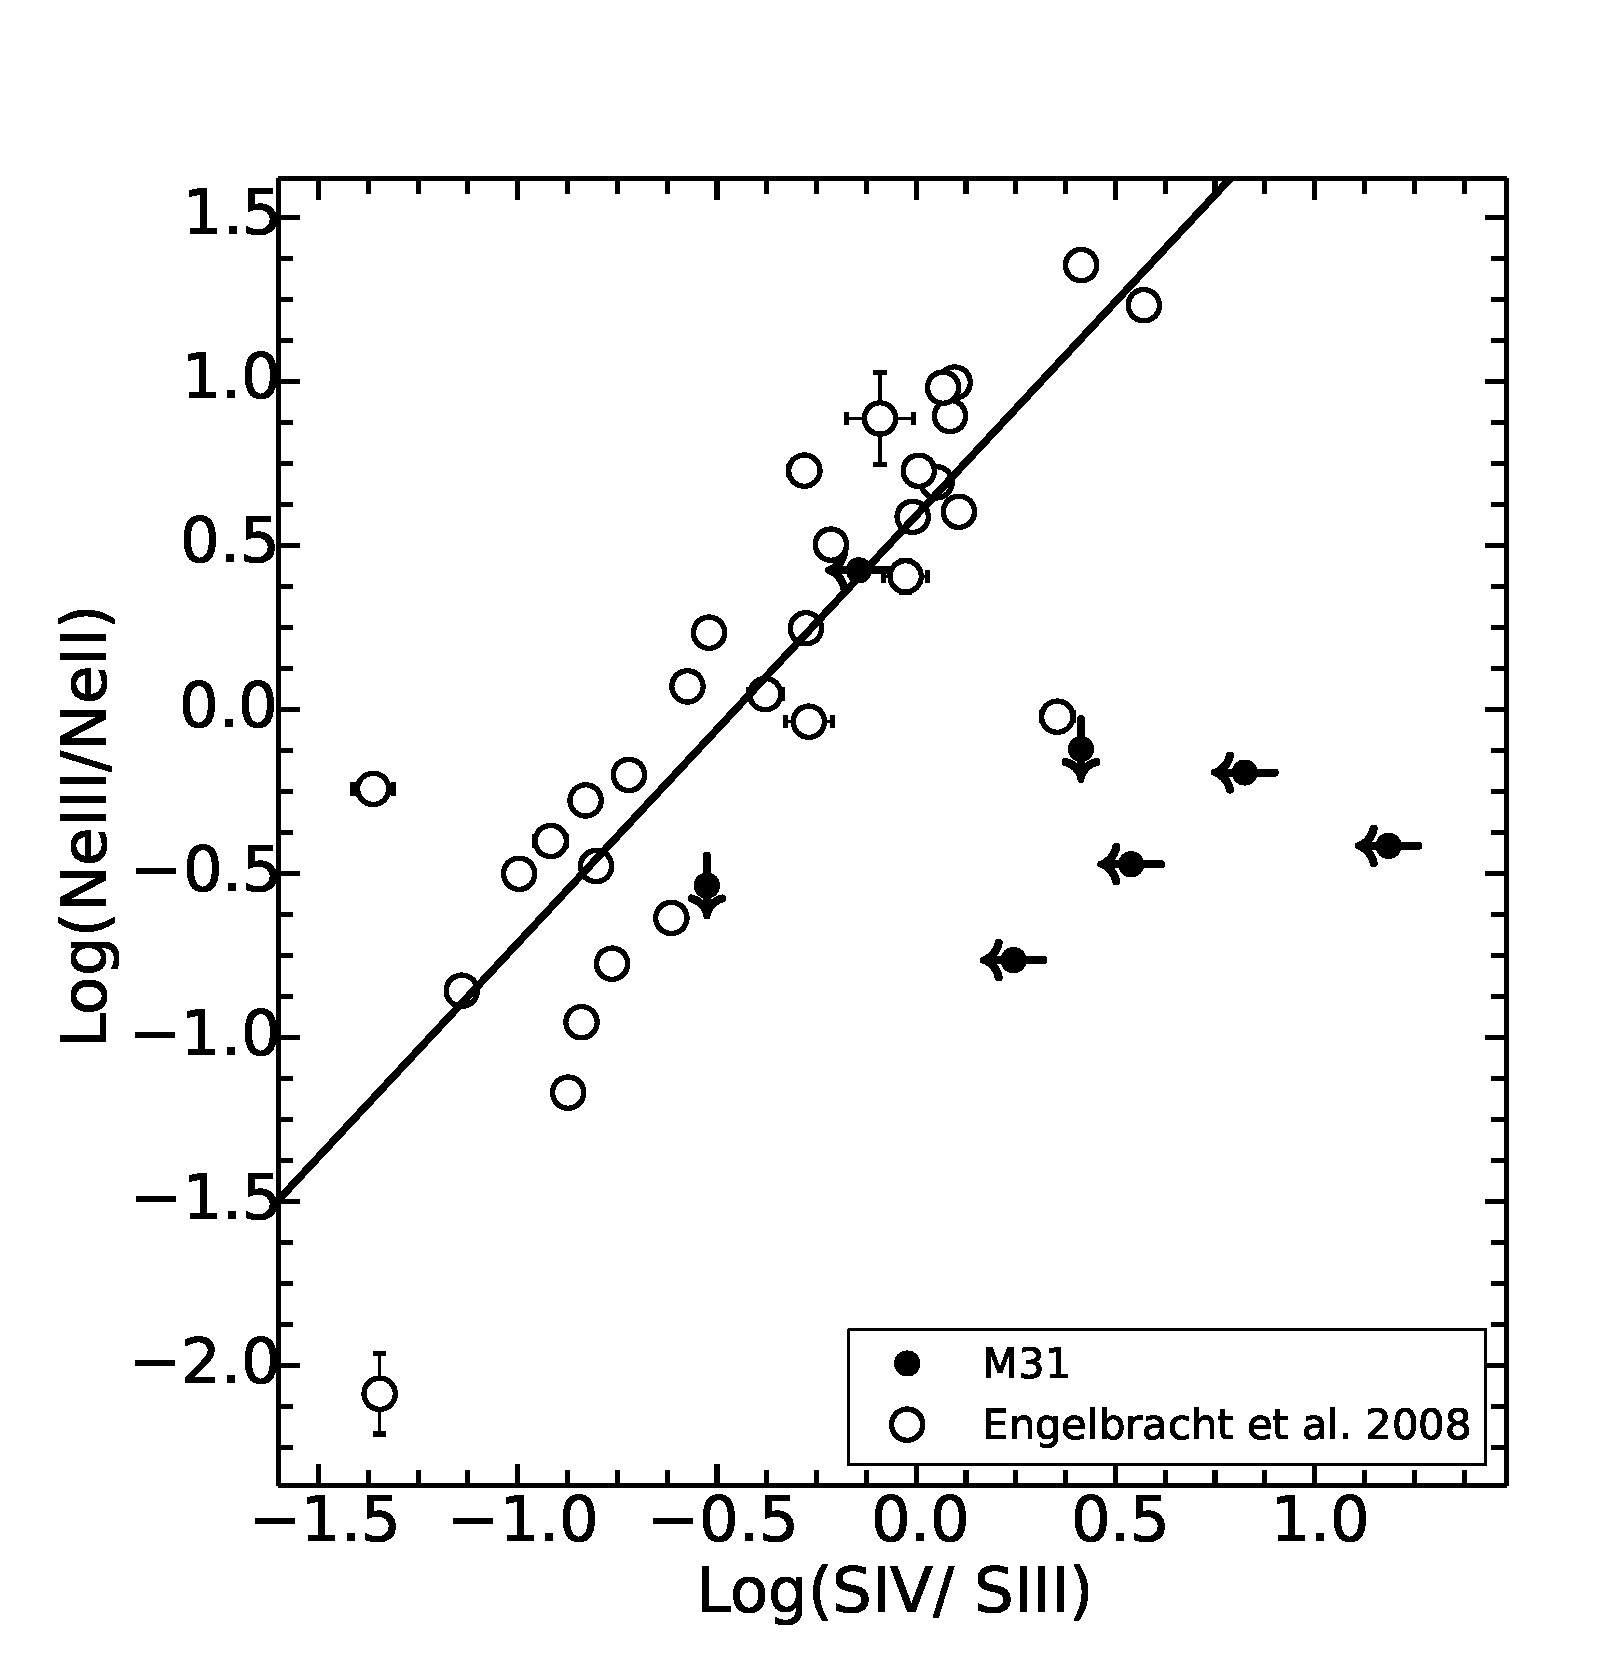
\includegraphics[scale=0.3]{./fig8.eps}
\caption{ Log([Ne~{\sc iii}]/[Ne~{\sc ii}])  vs log([S~{\sc iv}]/[S~{\sc iii}])  for the M31 regions in our sample (black dots) and  the starburst sample from \citet{Engelbracht_2008} (open dots). The straight line is the line of best fit for the starburst sample.
Upper limits are $3\sigma$.
}
\label{SvsNe}
\end{figure}

PAHFIT also returns the line strengths and uncertainties for atomic lines, listed in Table~\ref{Atomic}.
Not all lines were detected by PAHFIT, so we calculated upper limits for non-detected lines.%
\footnote{To find  the upper limits for the flux of missing atomic lines, we assumed the line to be a 
Gaussian profile with a FWHM as given by PAHFIT. The peak intensity was taken to be 3 times the RMS, where RMS is the root mean square of 
the noise at the position of a missing line.}
Line ratios of [Ne~{\sc iii}]/[Ne~{\sc ii}] and [S~{\sc iv}]/[S~{\sc iii}]~18 have been used as an indication of the radiation hardness, and
\citet{Engelbracht_2008} defined a combination of these two line ratios as a 'radiation hardness index (RHI)':
\begin{equation}
{\rm RHI} = \left( \log\frac{\textrm{[Ne~{\sc iii}] }}{\textrm{[Ne~{\sc ii}]}} + \left[0.71 + 1.58\log\frac{\textrm{{[S~{\sc iv}]}}}{\textrm{{[S~{\sc iii}]}}}\right]\right) /2
\end{equation}
\label{eq:rhi}
Here, 1.58 and 0.71 are the slope and intercept of the [Ne~{\sc iii}]/[Ne~{\sc ii}]  vs [S~{\sc iv}]/[S~{\sc iii}] plot (Figure \ref{SvsNe}) for the starburst sample from 
\citet{Engelbracht_2008}. The RHI has also been used by \citet{Gordon:2008lr} for M101 observations. 
Figure \ref{SvsNe}  compares the atomic line emission from the selected regions of M31 to the starburst galaxy sample;
although none of our spectra have detections of all four lines, our limits are mostly consistent with the wtrend.
We therefore compute the RHI using the first term of equation~\ref{eq:rhi} for the regions with missing S lines
and the second term for the regions with missing Ne lines.
Regions 2, 5, and 8 had detections of only one line per element, so we used the appropriate upper limits 
to calculate RHI for these spectra.


\begin{table*}
 \centering
 \begin{minipage}{100mm}
\caption{Atomic Emission Line Strengths$^a$}
  \begin{tabular}{l c c  c  c  c  c  }
  \hline
  {Region  }&{[Ar~{\sc ii}] }&{[Ar~{\sc iii}]  }&{[S~{\sc iv}]}&{[Ne~{\sc ii}]   }&{[Ne~{\sc iii}]   }&{[S~{\sc iii}]  }\\
{}&{\tiny{7.0 $\mu$m} }&{\tiny{9.0 $\mu$m }}&{\tiny{10.5 $\mu$m}}&{\tiny{12.8 $\mu$m  }}&{\tiny{15.5 $\mu$m } }&{\tiny{18.7 $\mu$m }} \\
 \hline 
 %  Pub_ID  ArII  ArIII  SIV  NeII  NeIII  SIII 
%  None  1e-15W/m2  1e-15W/m2  1e-15W/m2  1e-15W/m2  1e-15W/m2  1e-15W/m2 
       Bulge  & $<0.12$ & $0.17 \pm 0.03$ & $<0.11$ & $0.07 \pm 0.01$ & $0.025 \pm 0.006$ & $0.007 \pm 0.003$\\
    Region 1  & $<0.05$ & $<0.06$ & $0.020 \pm 0.004$ & $0.020 \pm 0.004$ & $<0.01$ & $0.008 \pm 0.001$\\
    Region 2  & $<0.05$ & $<0.06$ & $<0.02$ & $0.022 \pm 0.004$ & $<0.01$ & $0.003 \pm 0.002$\\
    Region 3  & $<0.15$ & $0.09 \pm 0.02$ & $<0.10$ & $0.03 \pm 0.01$ & $0.020 \pm 0.004$ & $0.015 \pm 0.003$\\
    Region 4  & $<0.04$ & $<0.04$ & $<0.02$ & $<0.02$ & $<0.01$ & $0.004 \pm 0.002$\\
    Region 5  & $<0.04$ & $<0.02$ & $<0.02$ & $<0.01$ & $0.009 \pm 0.004$ & $0.008 \pm 0.004$\\
    Region 6  & $0.02 \pm 0.01$ & $0.014 \pm 0.007$ & $<0.01$ & $<0.01$ & $0.019 \pm 0.002$ & $0.019 \pm 0.002$\\
    Region 7  & $<0.04$ & $<0.04$ & $0.008 \pm 0.003$ & $0.035 \pm 0.005$ & $<0.01$ & $0.027 \pm 0.004$\\
    Region 8  & $<0.04$ & $0.017 \pm 0.006$ & $<0.02$ & $<0.01$ & $0.041 \pm 0.002$ & $0.023 \pm 0.002$\\
    Region 9  & $0.09 \pm 0.04$ & $0.12 \pm 0.03$ & $<0.09$ & $0.13 \pm 0.01$ & $<0.04$ & $0.05 \pm 0.02$\\
 
\hline
 \label{Atomic}
\end{tabular}\\
{ $^a$Units are 10$^{-15}$~W~m$^{-2}$. Upper limits ($3\sigma$) are indicated with a $<$ mark.  }
\end{minipage}
\end{table*}



\section{Results and discussion}

\subsection{PAH intensities}
\label{sect:pah_ratios}

Both the 6.2 and 7.7~$\mu$m features are thought to be coming from ionized PAHs and the 11.3~$\mu$m feature from neutral PAHs. Therefore we expect to see a correlation between the intensities of 6.2 and 7.7~$\mu$m PAH features normalized by the 11.3~$\mu$m feature. In Figure \ref{PAHlines} we compare the PAH flux ratios of 7.7/11.3  and 6.2/11.3 features. The figure shows a good correlation between these two PAH line ratios, consistent with that of the SINGS sample shown by \citet{Smith:2007lr}.
A similar correlation was also reported by  \citet{Galliano2008} for a sample of galaxies and a handful of extended H{\sc ii} regions
and by \citet{Vermeij2002} for Galactic and Magellanic Cloud {\sc ii}regions. This provides evidence that the PAH emission from M31 is not unusual. 

\begin{figure}
\centering
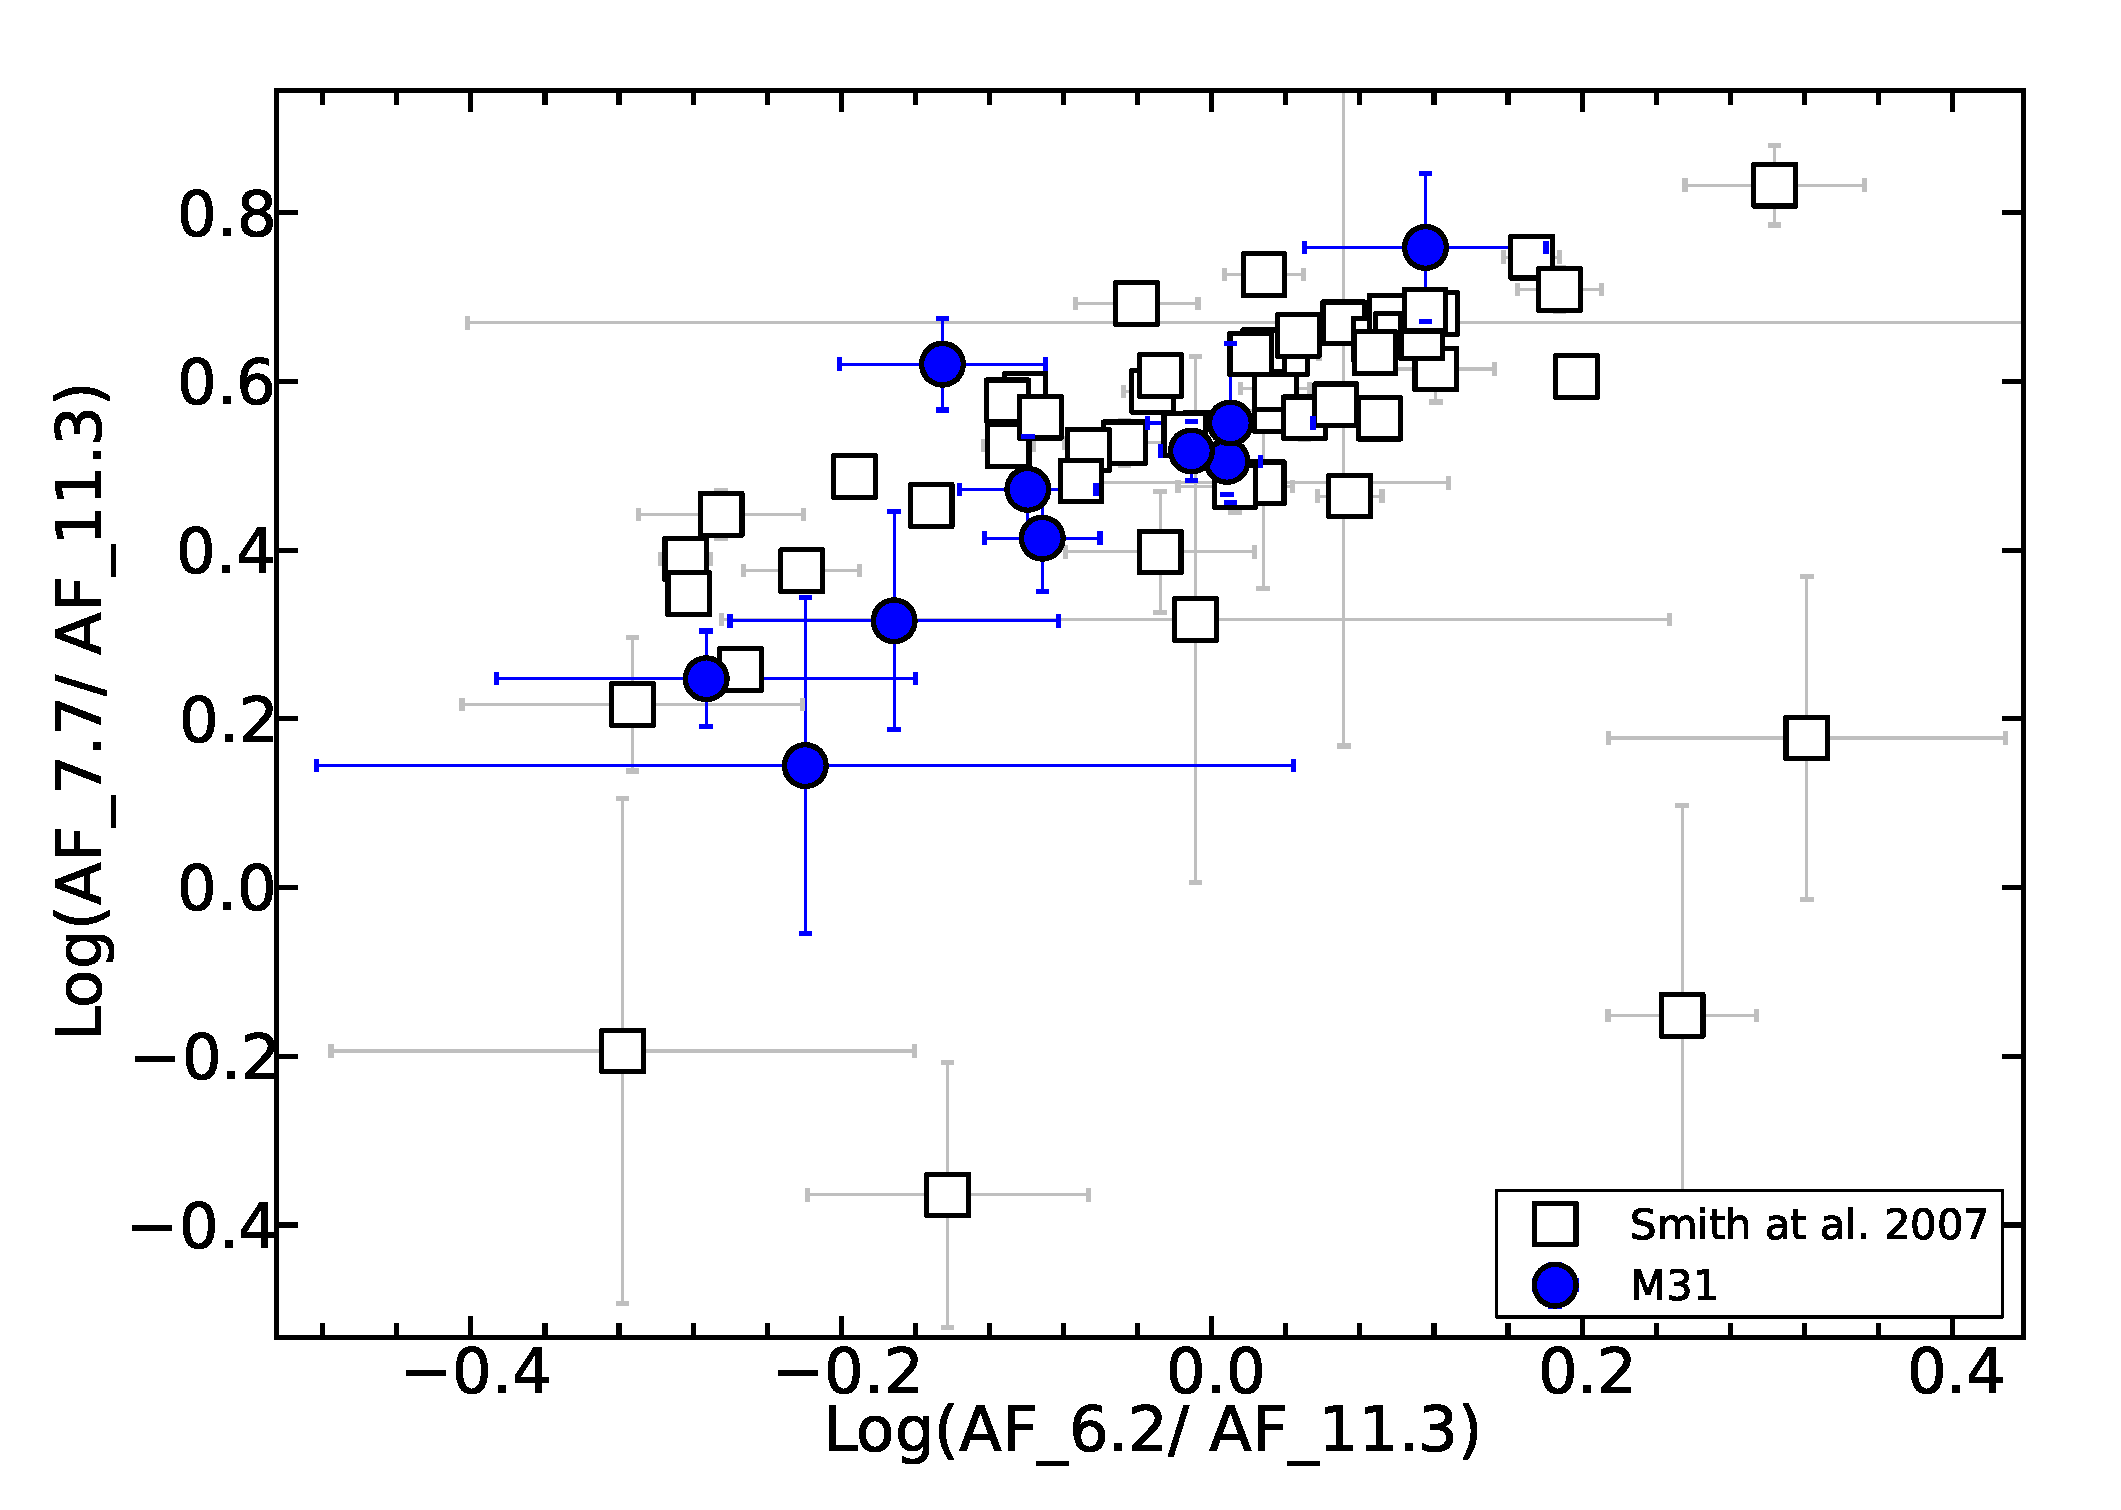
\includegraphics[scale = 0.25]{./SINGSnMy.eps}
\caption{Ratios of PAH feature fluxes (7.7~$\mu$m/11.3~$\mu$m versus 6.2~$\mu$m/11.3~$\mu$m) for 10 regions in M31.
Open squares represent the SINGs sample from \citet{Smith:2007lr}.
}
\label{PAHlines}
\end{figure}

\subsection{PAH equivalent widths versus radiation hardness}
\label{sect:eqw_rh}


\begin{figure}
\centering
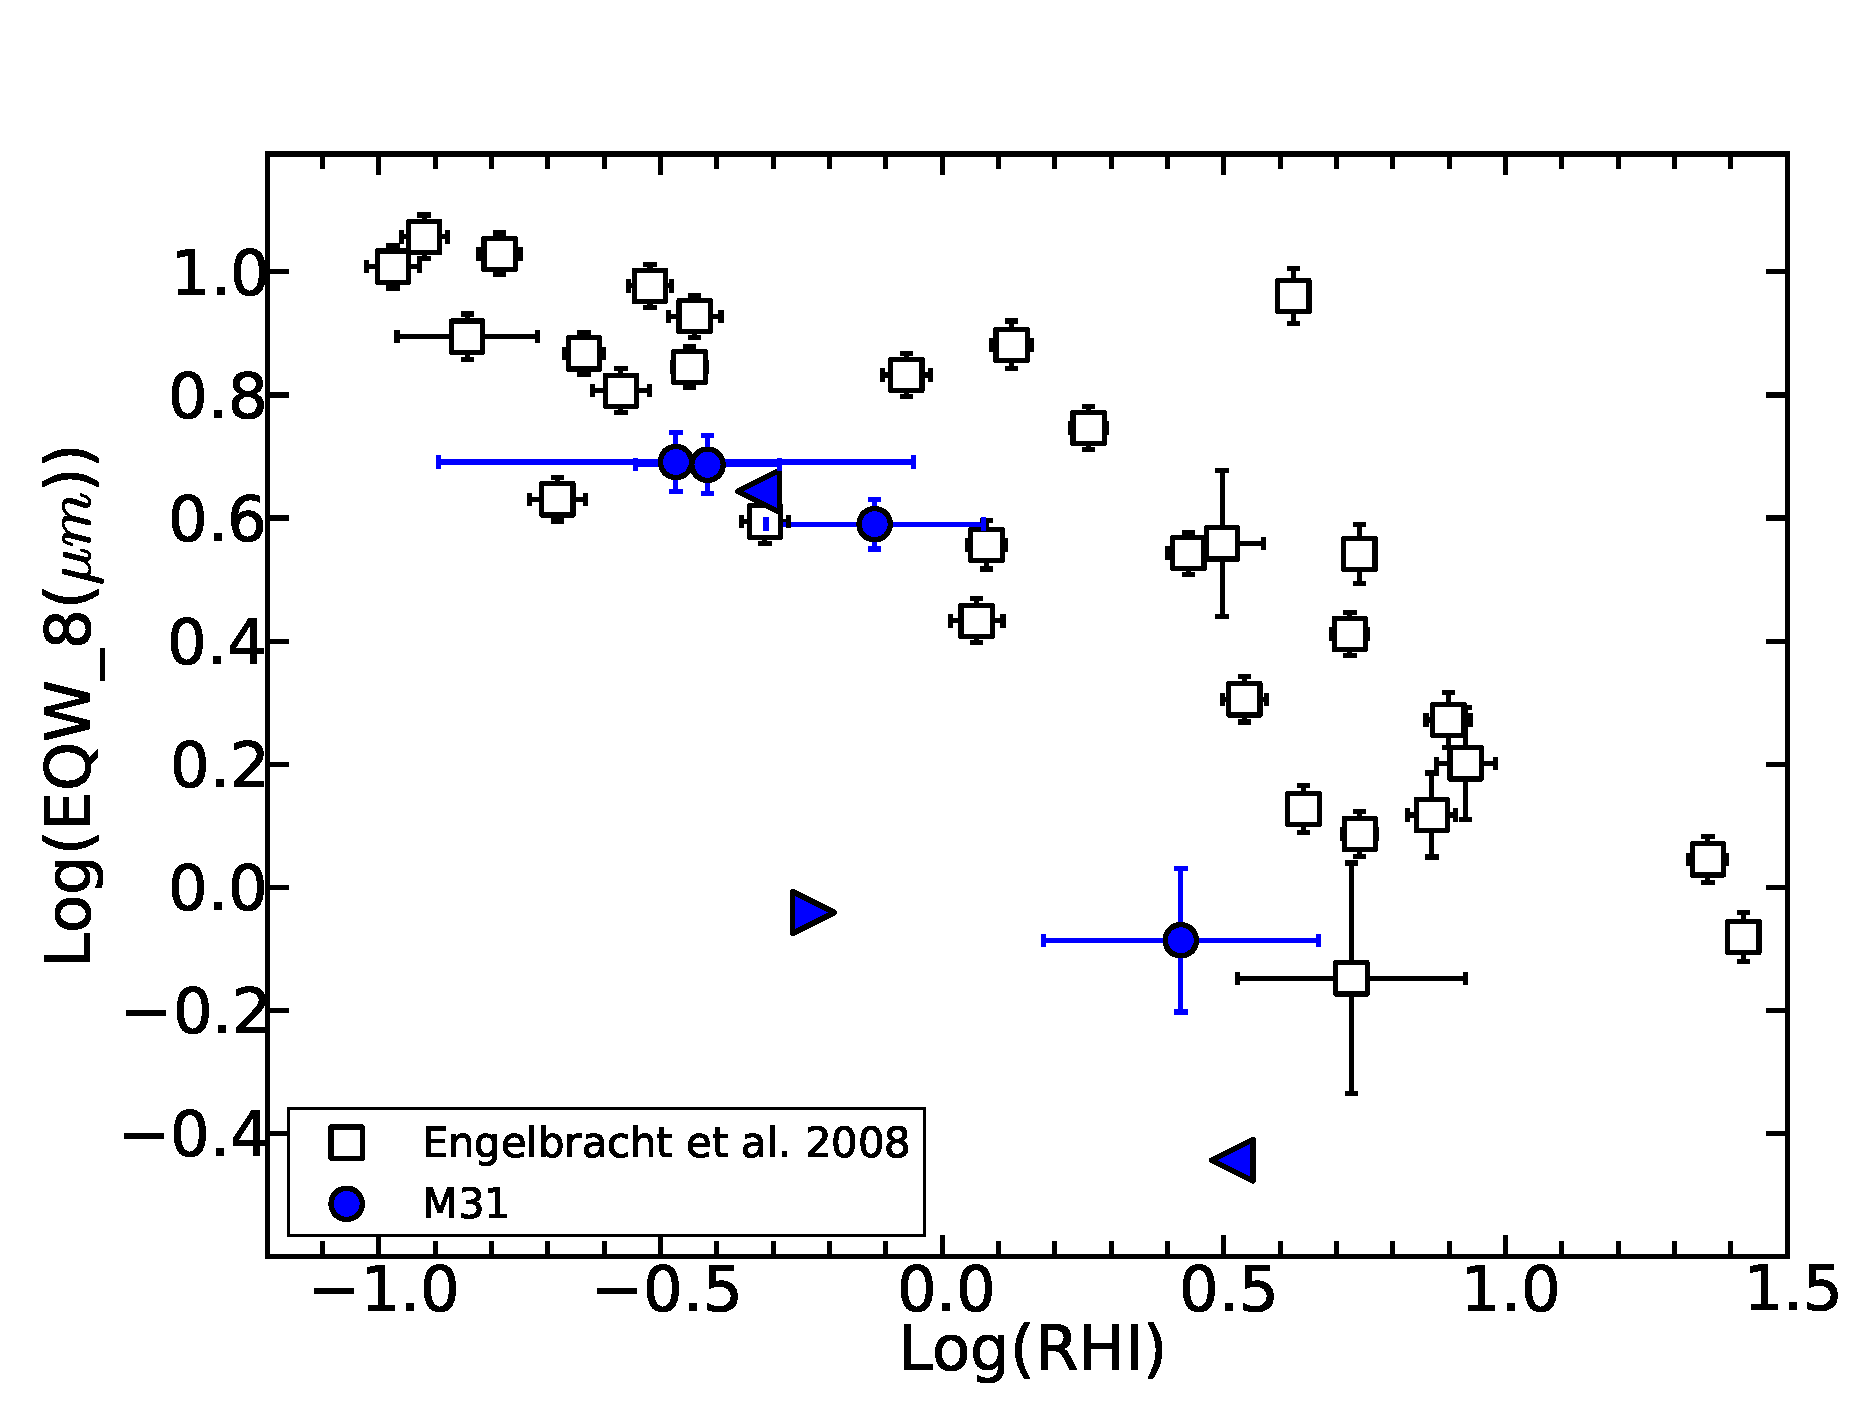
\includegraphics[scale=0.25]{./englvsmy.eps}
\caption{Equivalent width of the 8~$\mu$m PAH feature versus radiation hardness index (RHI) for the M31 sample (blue). 
The 8$\mu$m feature is a combination of the 7.7, 8.3 and 8.6~$\mu$m PAHFIT components. 
Open squares represent the starburst galaxy sample from \citet{Engelbracht_2008}. 
For M31 spectra with undetected lines, triangles represent upper (left-pointing triangles) and lower (right-pointing triangles) limits.}
\label{englII}
\end{figure}

\begin{figure}
\centering
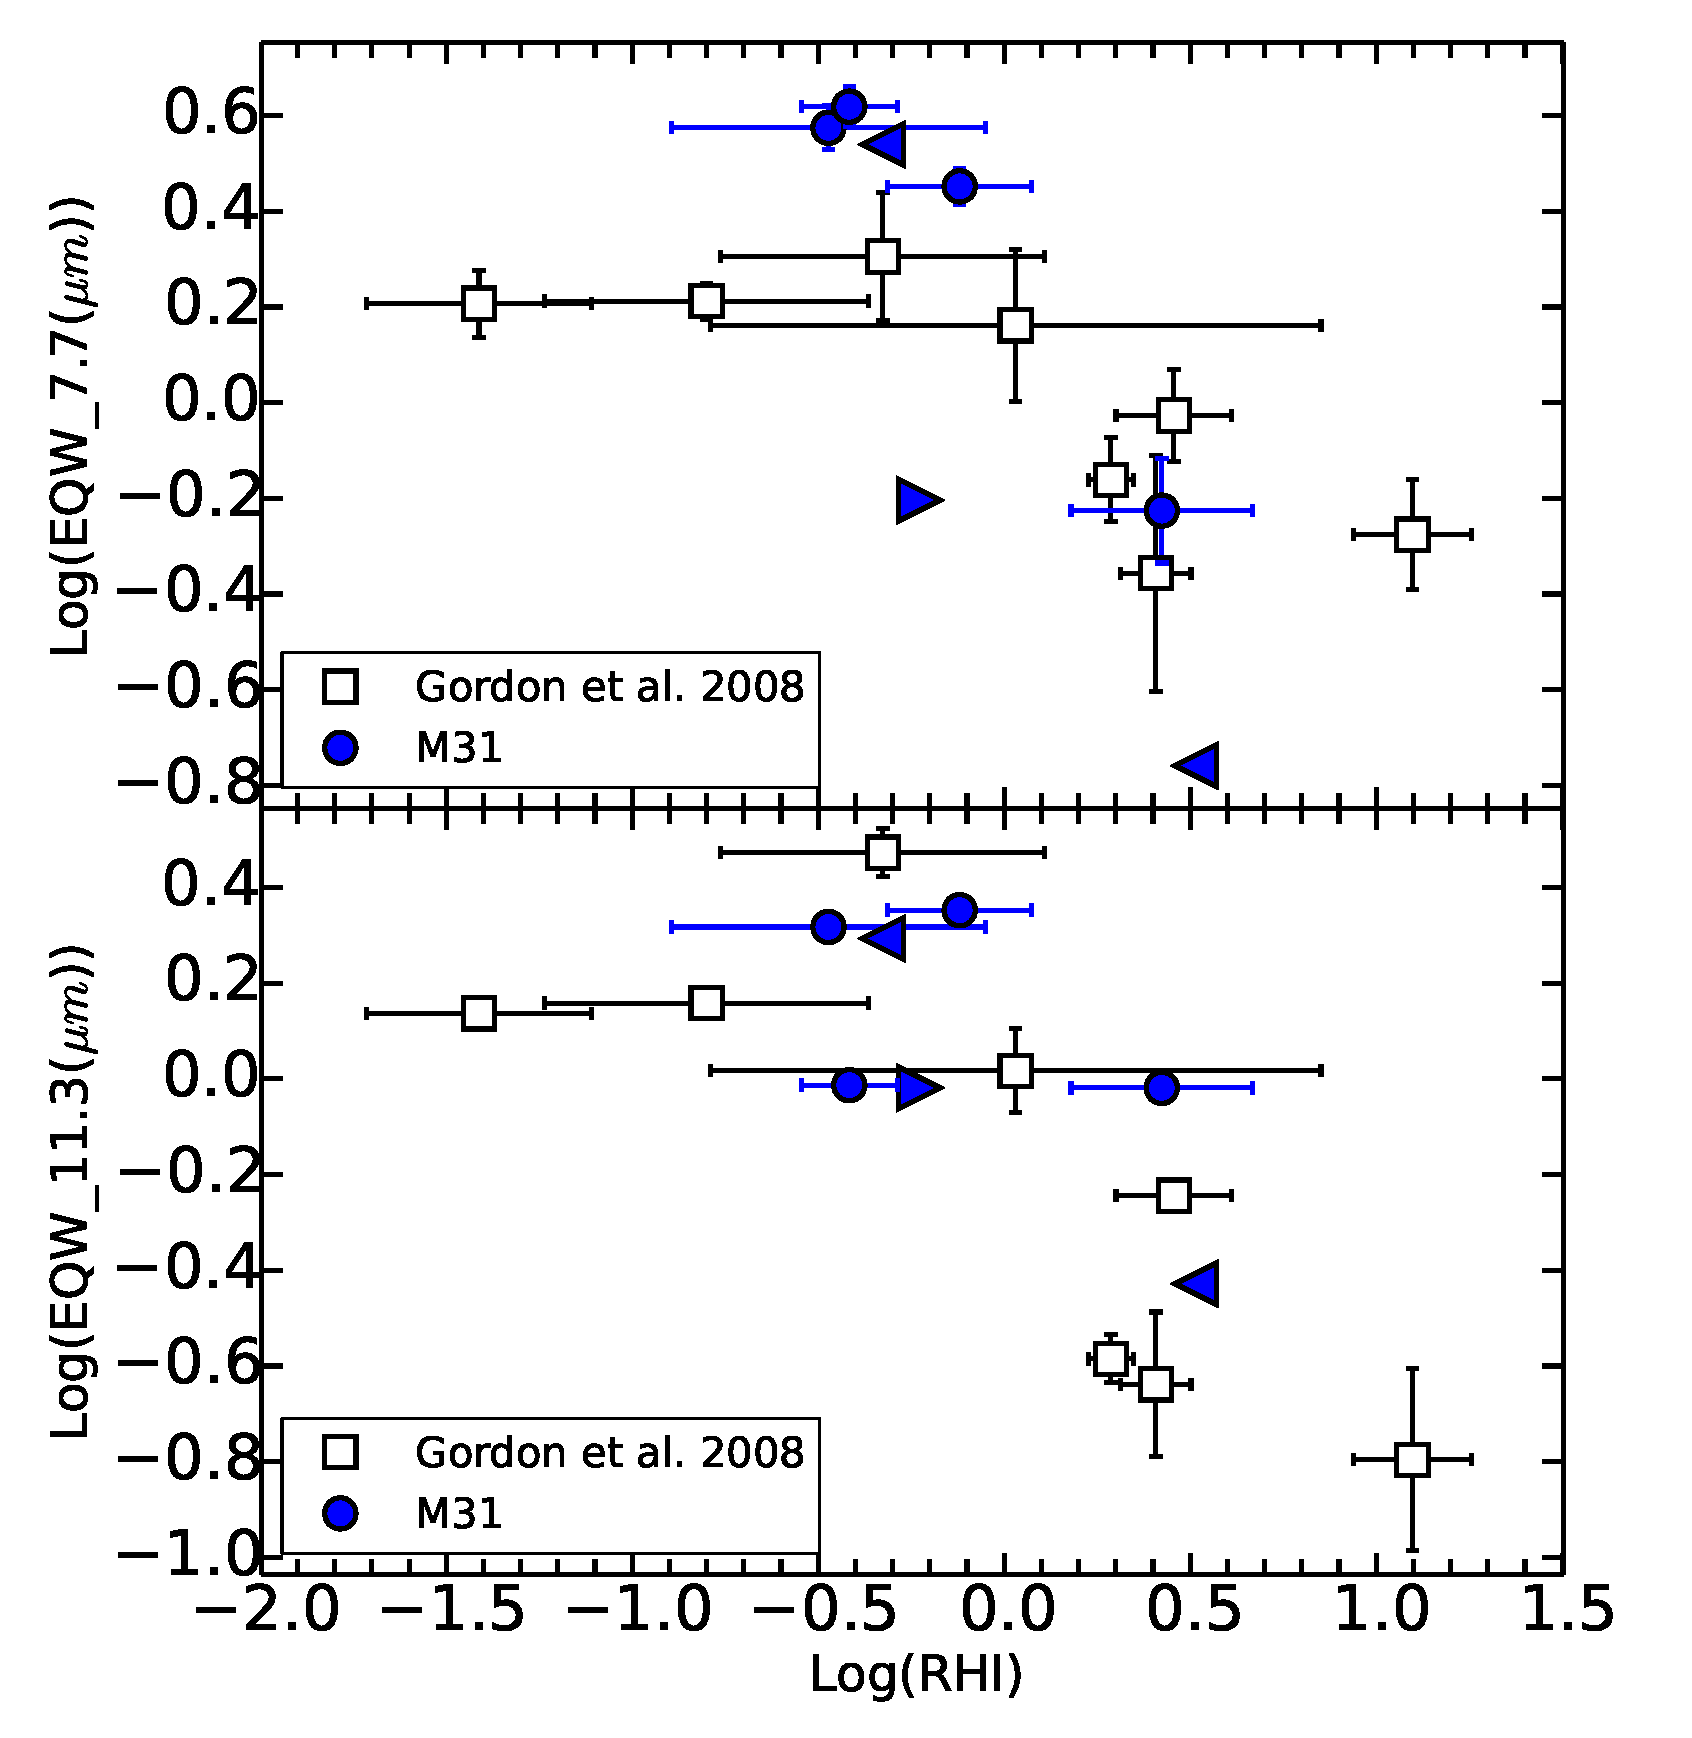
\includegraphics[scale=0.30]{./Gordvsmy.eps}
\caption{Equivalent widths of the normalized 7.7~$\mu$m PAH feature (top panel) and 11.3~$\mu$m PAH feature (bottom panel) versus 
radiation hardness index (RHI) for the M31 sample. Open squares represent the data from M101 by \citet{Gordon:2008lr}. 
The normalization was done by dividing each EQW by the weighted average over all regions in the respective samples. Triangles represent upper and lower limits.}
\label{gordII}
\end{figure}


As mentioned in the introduction, PAH equivalent widths tend to show an inverse correlation with radiation hardness. 
The equivalent widths of the M31 PAH features are compared with RHI in Figures~\ref{englII} and \ref{gordII}.
For reference, we also show the starburst sample of \citet{Engelbracht_2008}, which includes 66 nearby ($2<d<250$~Mpc)
star-bursting or star-forming galaxies selected to cover a wide range in metallicity ($7.1<12+\log{\rm[O/H]}<8.9$),
and the seven H~{\sc ii} regions in M101 observed by \citet{Gordon:2008lr}, which have $8.1<12+\log{\rm[O/H]}<8.8$.
To make a direct comparison with the M101 sample, we normalized the M31 EQWs in Figure~\ref{gordII} using the same procedure
as \citet{Gordon:2008lr}, dividing each EQW by the  weighted average over all regions in the respective samples. 
The equivalent widths seem to be decreasing with increasing radiation hardness, consistent with previous results. 
This also helps to confirm that the PAH emission in M31 is not unusual. 


\subsection{PAH equivalent widths versus metallicity}
\label{sect:eqw_met}

Many studies based on ISO and {\em Spitzer} observations have reported that PAH intensity decreases with decreasing metallicity \citep{Calzetti:2010fk}. 
In addition, these studies also report a sudden drop of EQWs of PAHs around $12+\log{\rm (O/H)} \approx 8.1$. 
This has been observed amongst different galaxies \citep{Engelbracht_2008} as well as within a single galaxy \citep{Gordon:2008lr}. 

Here we investigate the relation between the PAH features and the metallicity for the M31 regions in this paper. 
As a source of metallicity measurements, we used the work of \citet{Sanders_2011} who measured spectroscopic metallicities for
more than 250 H~{\sc ii} regions using strong line diagnostics.\footnote{\citet{Sanders_2011} considered several different
calibrations for abundance diagnostics. We use the results from the method they denote ``N06 N2''  \citep{Nagao2006} because
that method has the largest sample size.} Except for regions 5 and 8, all of our mapped regions contain an  H~{\sc ii} region measured by
 \citet{Sanders_2011}, and we give the corresponding metallicities in Table~\ref{regions}.
 For regions 5 and 8 we adopted metallicities from the radial metallicity profile of M31 given by
 \citet{Sanders_2011}. It is well known that there are systematic differences between different 
 methods used to measure metallicities, and those in the sample of \citet{Engelbracht_2008} 
 were obtained by the direct electron temperature method  \citep{Skillman1998}.
\citet{Mitchel2014} calculated the offset between direct and strong-line measurements for M31 H~{\sc ii} region to be 
$0.35\pm0.10$. In Figure \ref{metalicityVseqw} we have corrected for this offset  by subtracting 0.35 from our metallicities. 


\begin{figure}
\centering
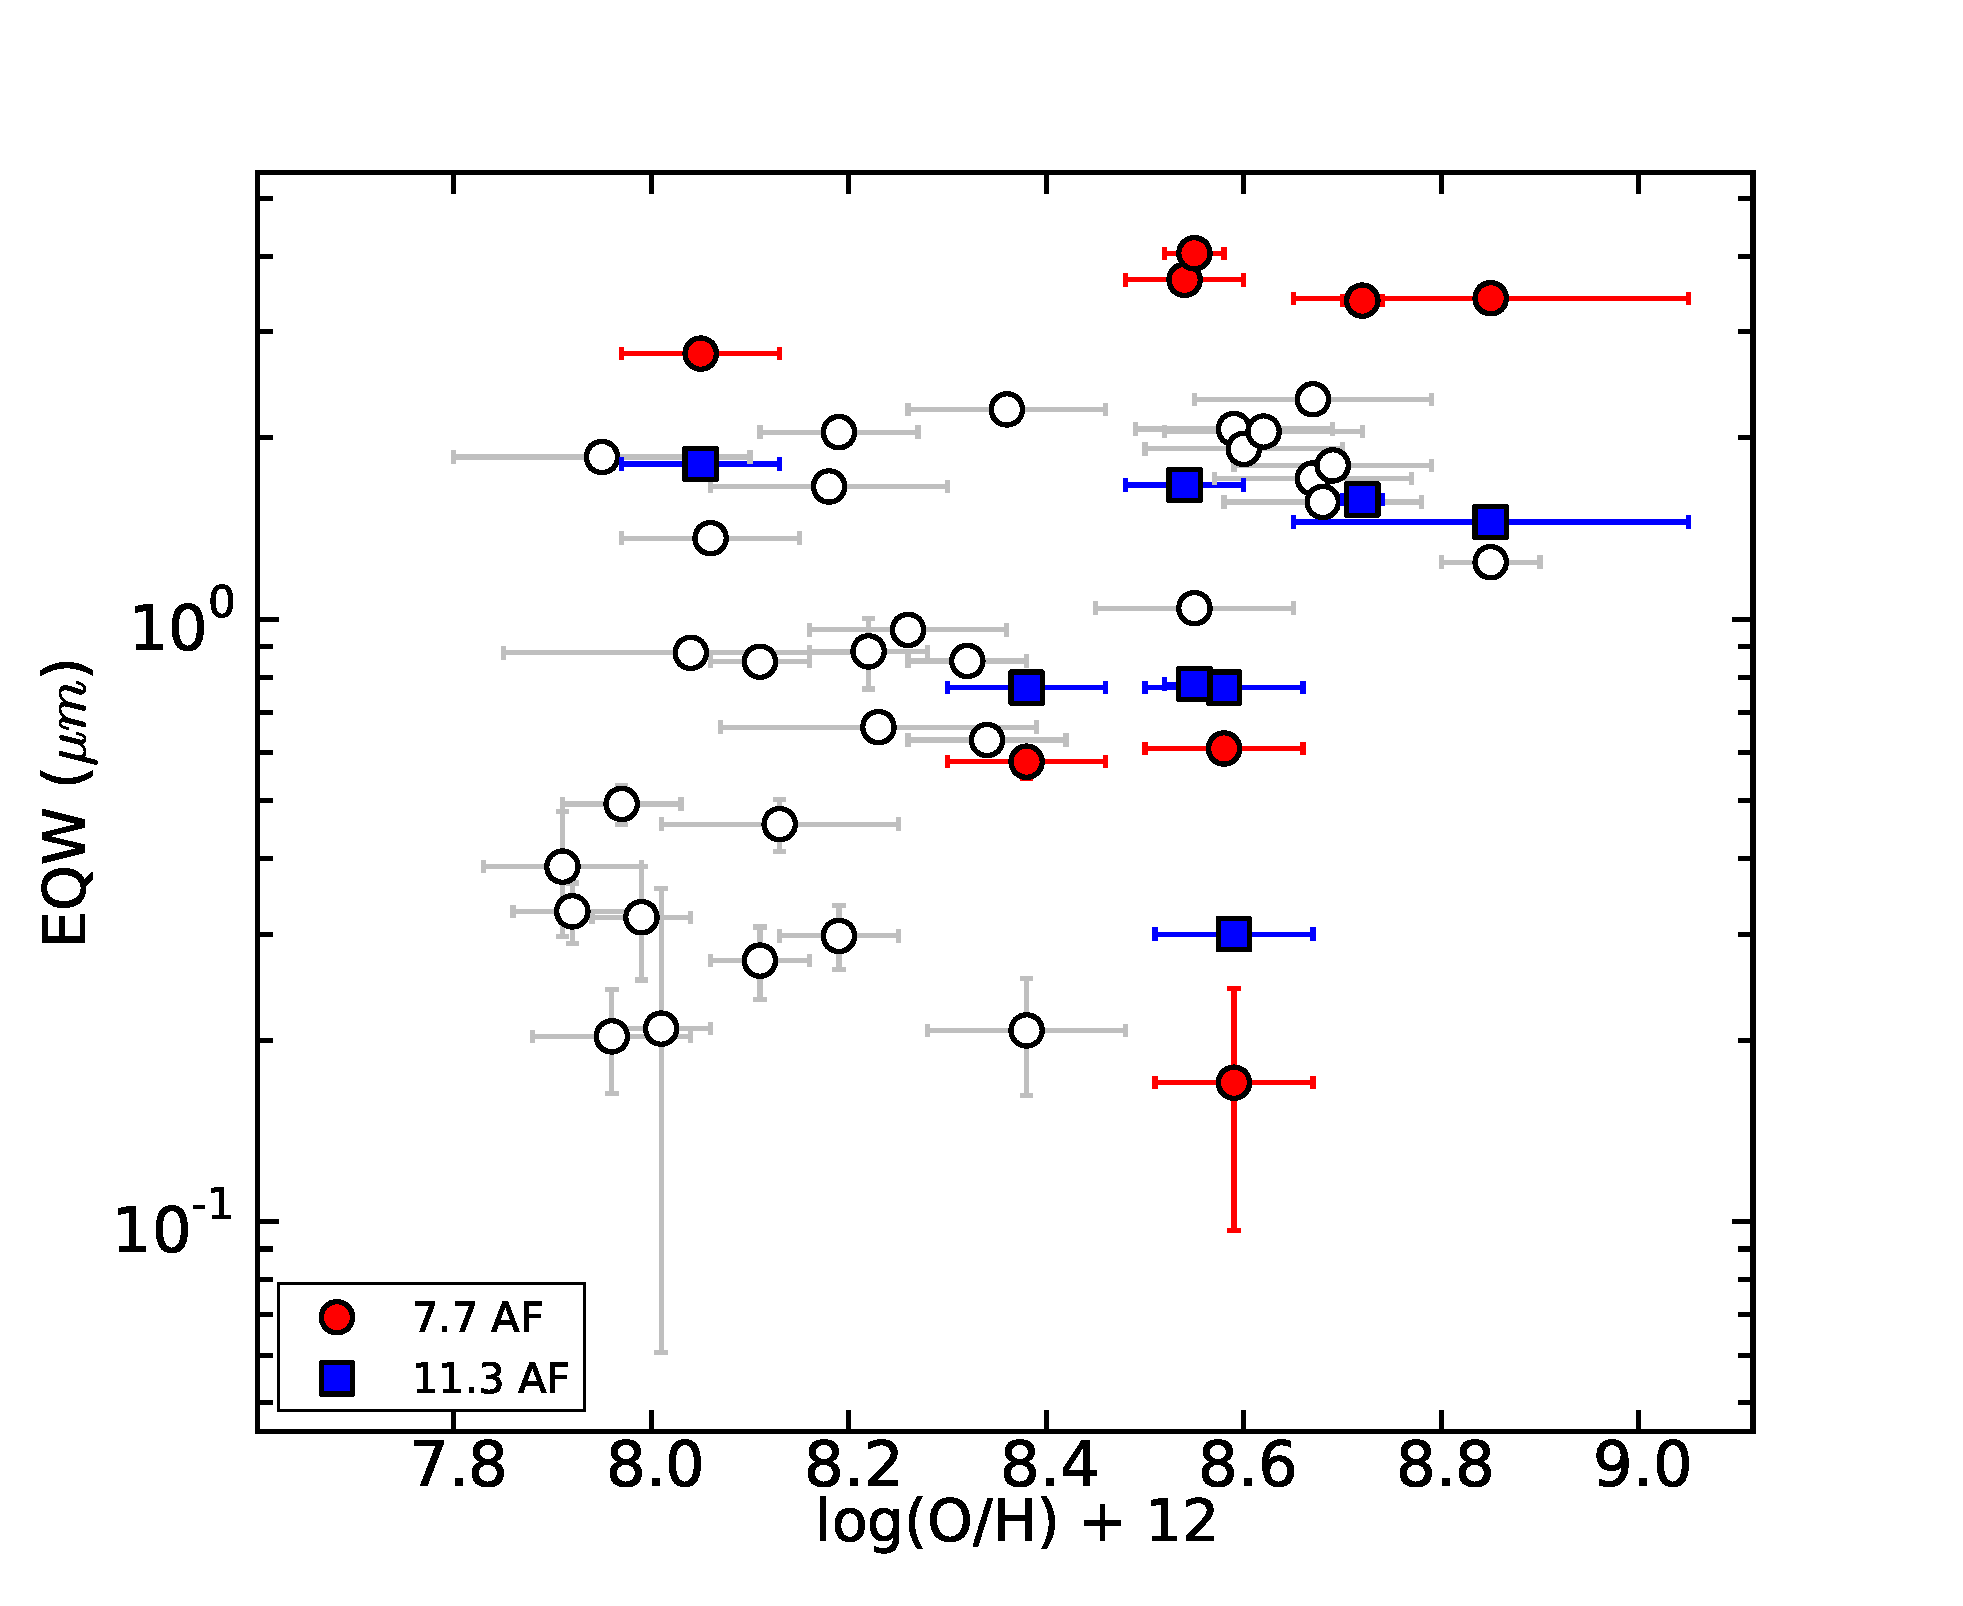
\includegraphics[scale=0.27]{./oxyvseqw.eps}
\caption{ PAH equivalent widths versus metallicity. EQWs of the 7.7~$\mu$m feature of the starburst sample from \citet{Engelbracht_2008} are plotted in open circles.}
\label{metalicityVseqw}
\end{figure}

Figure \ref{metalicityVseqw} plots the normalized EQWs of the PAH features are plotted versus the metallicity for our sample and the starburst 
galaxies of \citet{Engelbracht_2008}. The scatter in our sample is large, but the 	
equivalent widths of the 7.7 and 11.3~$\mu$m features are not inconsistent with those of \citet{Engelbracht_2008}. 
However, we do not have enough data from low-metallicity regions in M31 to observe the expected decrease of EQWs of PAH with the decreasing 
metallicity.  There do seem to be some outliers which can plausibly be due to the uncertainties  and the offset between different methods of calculating the metallicity.  
%SPW: Sec 4.2 par 4: while there's no metallicity dependence, 1 region has very low PAH.    Any idea why?  Is it just stellar light contamination, or is something fundamental happening?

\subsection{Dust properties of the nucleus}
\label{sect:nucleus}

%
%I guess the nuclear spectrum is in your Figure 15 - why did you not try to fit it with PAHFIT too?  It looks to me like it has a weak 20um silicate bump too.
% Why not include the nuclear region in Tables 2,3&4?  I did not understand the reason for leaving it off.  Also please add the limit for the [Ne V] detection - it might still be a useful ratio with [Ne II] and the PAH lines.  It looked to me like there was some hint of the H2 12.28um line in some regions.... maybe add that limit too, though I was surprised

\begin{figure*}
\centering
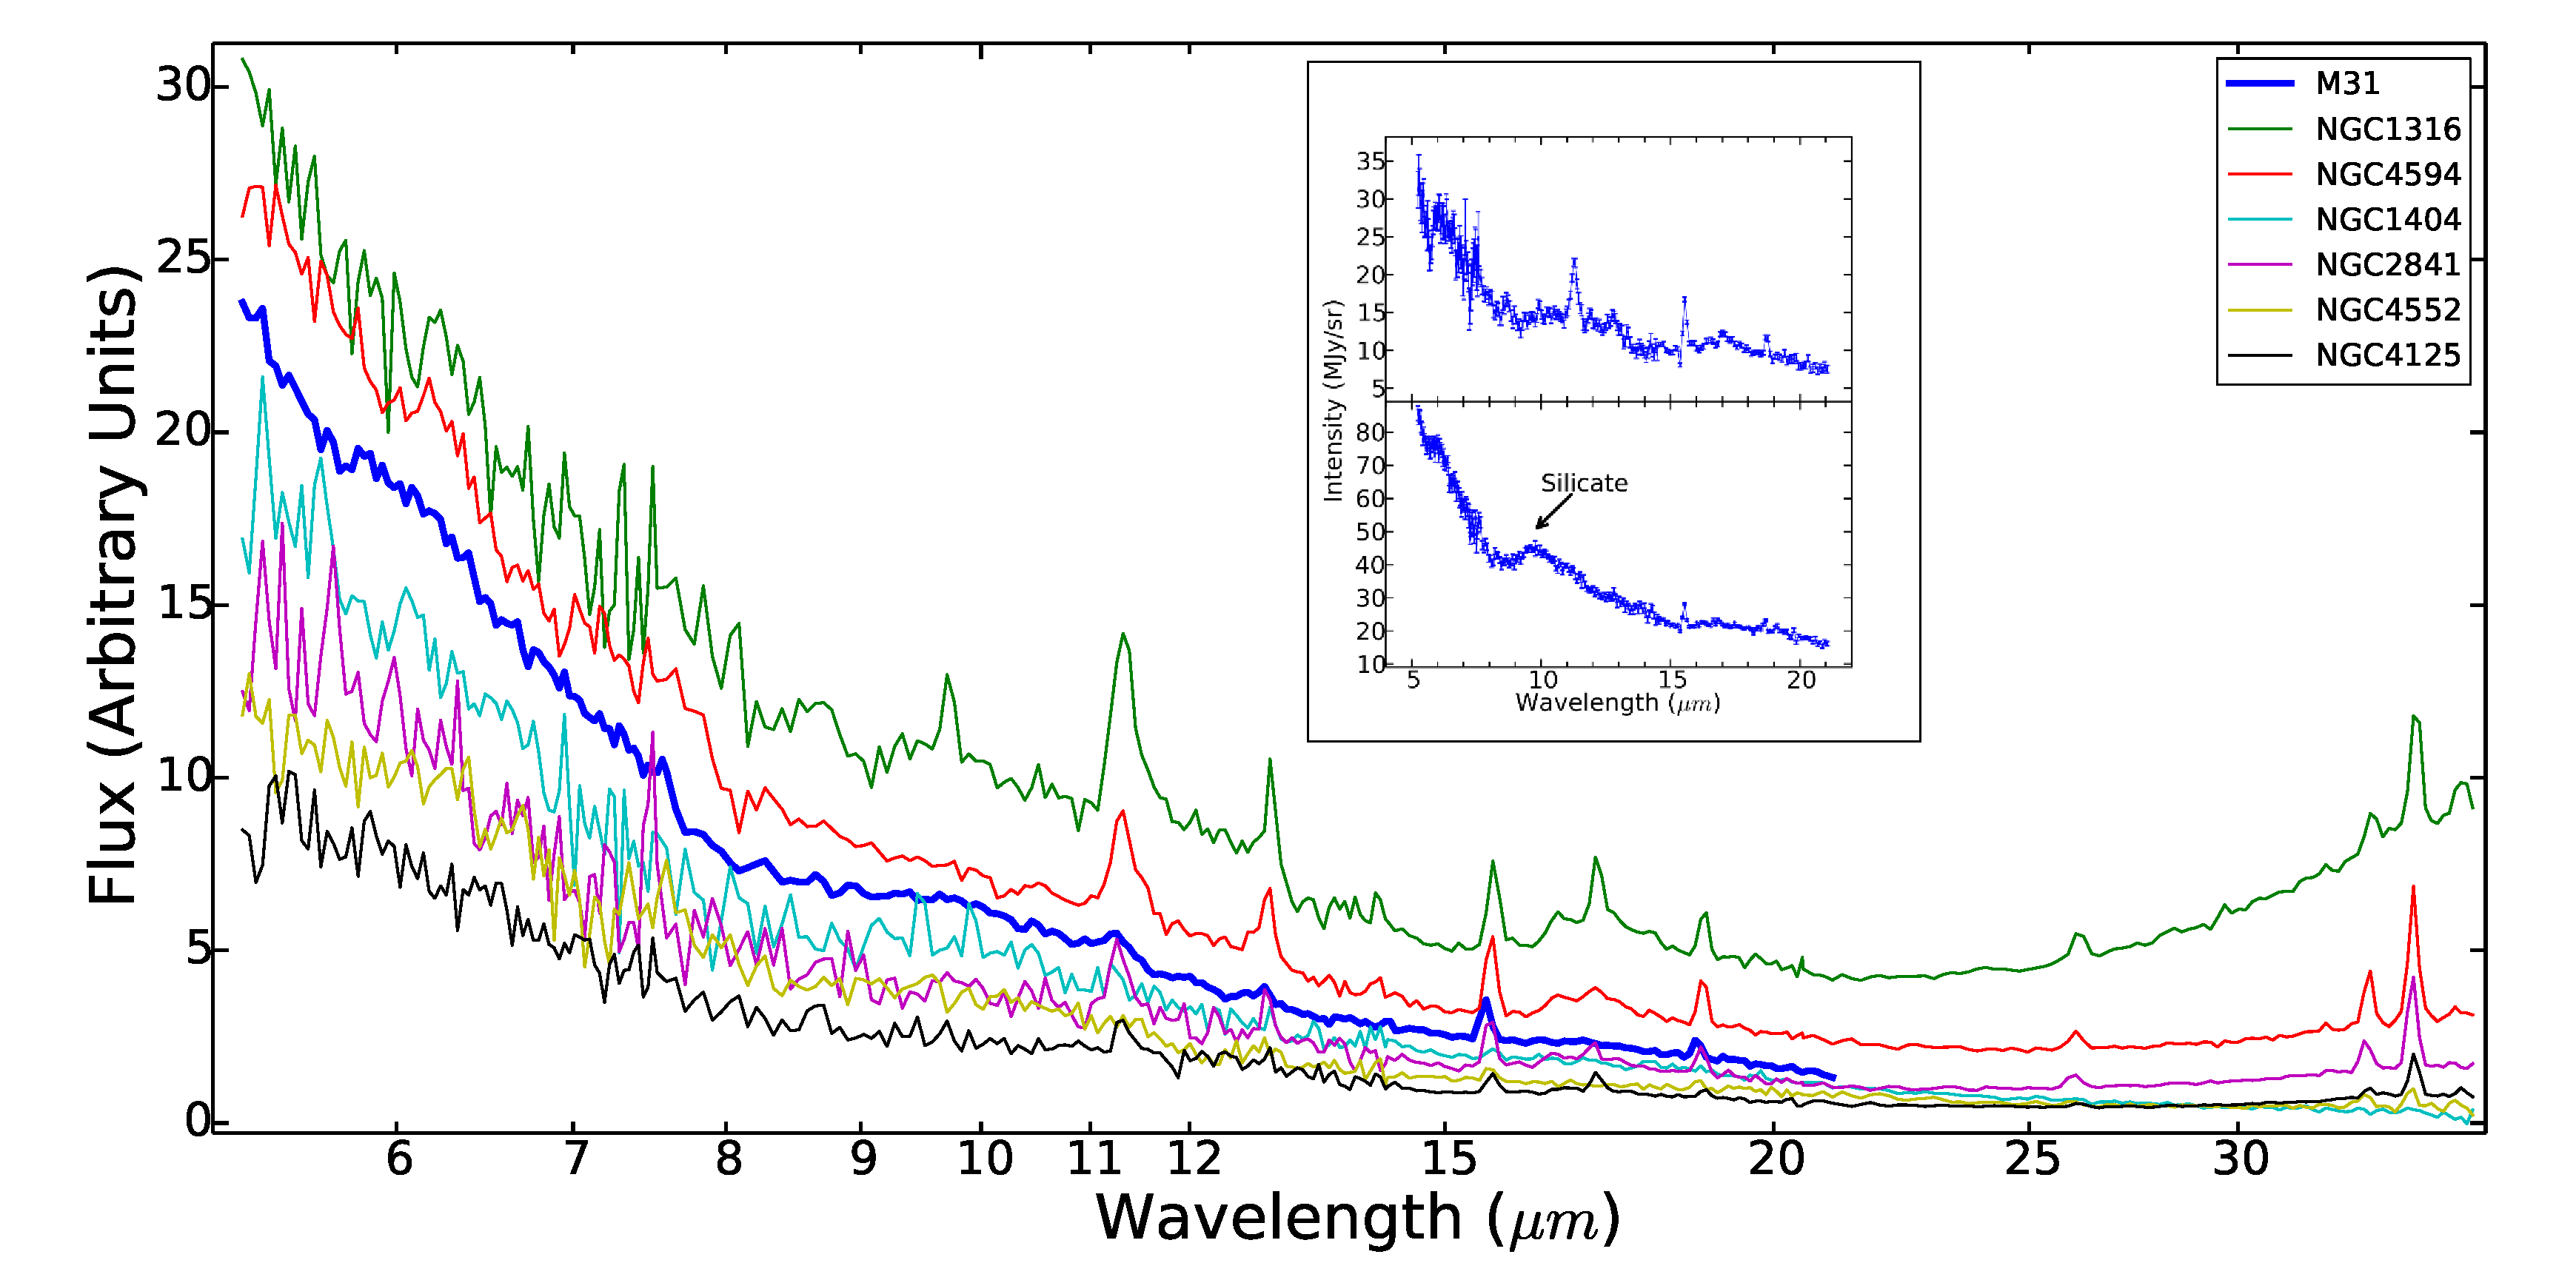
\includegraphics[height = 8 cm]{./SINGSspec.eps}
\caption{Mid-infrared spectrum of the nucleus of M31 (blue) over-plotted with spectra extracted close to the nuclei of 6 nearby galaxies which have 
AGN activity \citep{Smith:2007lr}. NGC 4552, NGC 1404 and NGC 4125 are elliptical galaxies and NGC 4594 and NGC 2841 are spiral galaxies. 
NGC 1316 is a lenticular galaxy. The inset shows the spectra extracted from the centre region of the M31 nucleus (bottom) and from the north region (top) 
shown in Figure \ref{nuc11}.}
\label{smithspec}
\end{figure*}

The mid-infrared spectra of the nucleus from both {\em Spitzer} and ISOCAM (Figure~\ref{ISOnIRS}) show similar characteristics: a blue
continuum, PAH features weak or absent at 6--8~$\mu$m  but detectable at 11.3~$\mu$m, and detectable atomic fine structure lines.
Comparing the M31 nuclear spectrum with the nuclear spectra from the SINGS sample given by \citet{Smith:2007lr}, we found
six other galaxies with similar spectral shapes, including three elliptical galaxies, two spirals, and a lenticular.
The IRS spectra for the SINGS galaxies were extracted over areas ranging from 2 to 8 kpc$^2$, whereas the M31
nucleus spectrum covers a much smaller area (0.02~kpc$^2$).
The SINGS papers \citep{kennicutt03,Smith:2007lr, moustakas2010} are in some disagreement over the
exact nuclear spectral types of these six galaxies. All are classified as some form of low-luminosity AGN
such as Seyfert or LINER \citep[luminous AGN were intentionally omitted from the SINGS sample][]{kennicutt03}, but they are
by no means the only LLAGN in the SINGS sample.
Figure~\ref{smithspec} shows the M31 nuclear spectrum with the comparison SINGS spectra.
The spectrum extracted  from the North region (Figure \ref{smithspec}, inset) shows a strong 11.3~$\mu$m peak 
and no significant emission from 6--8~$\mu$m features. These characteristics are shared by
the M81 nuclear spectrum presented by \citet{Smith2010}, although that spectrum has little stellar continuum and a very strong [Ne {\sc ii}]~12.8~$\mu$m line. 


As discussed by  \citet{Smith:2007lr} and \citet{Smith2010}, inferring the suppression of 6--8~$\mu$m PAH features compared
to the 11.3~$\mu$m feature must be done with caution, since the 6--8~$\mu$m features are more susceptible to dilution by the stellar
continuum. Such suppression could have several causes: destruction of small or charged PAH molecules by an AGN,
or weak ultraviolet continuum indicating lack of star formation \citep{Smith:2007lr}. In the latter case, the AGN is not the cause of
the suppressed  6--8~$\mu$m features, but rather is only detected when the nuclear star formation rate is low.
An implication of low star formation in the centre of M31 is consistent
with previous work: although \citet{Melchior2013} found a significant amount of cold gas in the centre of the galaxy, this gas does not
appear to be associated with current star formation. In modelling the far-infrared spectral energy distribution, \cite{Groves2012} found that  
the old stellar population in the M31 bulge is sufficient  to heat the observed dust; no young stellar population is needed.


Examining the spatial distribution of the mid-infrared emission in the M31 nuclear region provides additional clues
to the nature of the emitting sources. Figure~\ref{nuc11} shows that most of the 11.3~$\mu$m comes from a region to the
north of the nucleus, while the silicate emission (Figure~\ref{silicate}) is centred on the nucleus itself.  Figure \ref{smithspec}
compares the spectra extracted from these two regions (see~Section~\ref{sect:obs_nuc}). Silicate emission is not very common in
integrated spectra of galaxies \citep{Spoon2007} but is seen in luminous quasar spectra \citep{Hill14} and, as mentioned above, in the
spectrum of the M81 nucleus. We computed the linear slope parameter  defined by \citet{Smith2010},
$\gamma810 =[F_{\nu}(10\mu{\rm m}) -F_{\nu}(8\mu{\rm m})]/2F_{\nu}(9\mu{\rm m}) $, for the M31 nucleus and
found $\gamma810 =-0.08\pm 0.06$.  This is 
%HAS: It might be useful to tabulate the masses of the black holes in each of the 6 comparison galaxies, to see whether spectral similarities (or differences) can be attributed to the quiescent AGN, as you suggest, of whether circumnuclear star formation or other things might play some role.


Does detection of silicate emission in the M31 nuclear spectrum imply the detection of an active nucleus?
In the unified model of AGNs, an obscuring torus viewed face-on would be expected to show silicate emission
\citep{AGNtypes1995, AGNref}; however such a view would also be expected to show forbidden atomic lines such as [Ne~{\sc v}] and [S~{\sc iv}],
not seen in the M31 spectrum. Alternatively, \citet{Mason2012} explained that low-luminosity AGNs cannot 
host a Seyfert-like obscuring torus because of their optically thin dust and low dust-to-gas ratio, but can show
the silicate emission that originates in the optically thin hot dust around the torus.  The first detection of such silicate emission was 
reported by \citet{Sturm2005} from the low-ionization nuclear emission-line region (LINER) galaxy NGC~3998, and 
\citealt{Mason2012}  observed that this 9.7~$\mu$m silicate emission is present in many LLAGNs. 
We computed the bolometric luminosity of the M31 nucleus  to be (**value goes here**) erg~s$^{-1}$ using the 12~$\mu$m flux 
and the method described in \citet{luminosity}. This value is close to that of other LLAGNs (**and consistent with the X--ray value?**)


\section{Summary and conclusions}

We  obtained {\em Spitzer}/IRS spectral maps of 12 regions within M31 covering wavelengths 5--21~$\mu$m. 
The spectra from those regions, except for the nucleus, are similar to spectra obtained from other nearby  star-forming galaxies. 
Early  ISOCAM observations  towards 4 regions of M31 showing a suppression 
of the 6--8~$\mu$m features and an enhancement of  the 11.3~$\mu$m feature  \citep{1998Cesarsky} 
were likely affected by the background subtraction methods applied.

The PAH intensities in M31 regions show a decreasing trend with increasing radiation hardness, consistent with previous 
results from other nearby galaxies. The distribution of PAH EQWs with metallicity is well within the range of the starburst galaxy sample of \citet{Engelbracht_2008}. 
We did not have enough data from low-metallicity regions of M31 to observe the decreasing trend of EQWs at low metallicities which is visible in other galaxies.

Mid-infrared spectra from near the nucleus of M31 show either suppressed 6--8~$\mu$m features and a strong 11.3~$\mu$m feature
(15\arcsec off-nucleus) or silicate emission around 9.7~$\mu$m  (on-nucleus). 
The nuclear spectrum is similar to that of six other nearby galaxies known to have low-luminosity AGN activity. This could strengthen the
suggestion by \citet{Smith:2007lr} that low $L(7.7\mu{\rm m})/L(11.3\mu{\rm m})$ is an indicator of low luminosity AGN,
but this feature ratio could also be due to a lack of ionized PAHs. The nuclear silicate emission is another possible AGN indicator.
The 12~$\mu$m luminosity can be used wto estimate a bolometric luminosity for the M31 nucleus of $10^{39}$~erg~s$^{-1}$.


\section*{Acknowledgements}


DH acknowledges D. Stock, K. Sandstrom and S. Lianou for fruitful discussions and technical support. 
We acknowledge support from NSERC Discovery Grants to PB and EP and an NSERC Discovery Accelerator Grant to EP. 
This work is based on observations made with the {\em Spitzer} Space Telescope, which is operated by the 
Jet Propulsion Laboratory, California Institute of Technology under a contract with NASA.
This research has made use of NASA's Astrophysics Data System.



\bibliographystyle{mn2e}
\bibliography{reference}{}

\bsp

\label{lastpage}

\end{document}
